\documentclass[tog]{acmsiggraph}

\usepackage{mystyle}

\usepackage{MyMnSymbol} % fixes underbrace command
\usepackage{xcolor}
\usepackage{microtype}
\usepackage{pbox}

\TOGonlineid{0372}
\TOGvolume{0}
\TOGnumber{0}
\TOGarticleDOI{1111111.2222222}
% \TOGprojectURL{}
% \TOGvideoURL{}
% \TOGdataURL{}
% \TOGcodeURL{}

%

\title{Convolutional Wasserstein Distances: \\ Efficient Optimal Transportation on Geometric Domains}

\author{Justin Solomon \\ Stanford University\\\ \\ \and Fernando de Goes \\ Pixar Animation Studios \and Gabriel Peyr\'e \\ CNRS \& Univ. Paris-Dauphine \and Marco Cuturi \\ Kyoto University \and Adrian Butscher \\ Autodesk, Inc. \and Andy Nguyen \\ Stanford University \and Tao Du \\ Stanford University \and Leonidas Guibas \\ Stanford University}
\pdfauthor{Justin Solomon, Fernando de Goes, Gabriel Peyr\'e, Marco Cuturi, Adrian Butscher, Andy Nguyen, Tao Du, Leonidas Guibas}

\keywords{Optimal transportation, Wasserstein distances, entropy, displacement interpolation.}

\begin{document}

%% \teaser{
%%   \includegraphics[height=1.5in]{images/sampleteaser}
%%   \caption{Spring Training 2009, Peoria, AZ.}
%% }

\teaser{
% }\begin{figure*}[t]\centering
\centering
\vspace{-.25in}
\includegraphics[width=\linewidth]{figures/teaser/cowducktorus.pdf}
\caption{Shape interpolation from a cow to a duck to a torus via convolutional Wasserstein barycenters on a $100\!\times\!100\!\times\!100$ grid, using the method at the beginning of \S\ref{sec:applications}.}\label{fig:teaser}\vspace{-.05in}
%\end{figure*}
}

\maketitle

% !TEX root = ../convolutional_w2.tex

\begin{abstract}
This paper introduces a new class of algorithms for optimization problems involving optimal transportation over geometric domains.  Our main contribution is to show that optimal transportation can be made tractable over large domains used in graphics, such as images and triangle meshes, improving performance by orders of magnitude compared to previous work.  To this end, we approximate optimal transportation distances using entropic regularization.  The resulting objective contains a geodesic distance-based kernel that can be approximated with the heat kernel. This approach leads to simple iterative numerical schemes with linear convergence, in which each iteration only requires Gaussian convolution or the solution of a sparse, pre-factored linear system.  We demonstrate the versatility and efficiency of our method on tasks including reflectance interpolation, color transfer, and geometry processing.
\end{abstract}


\begin{CRcatlist}
%  \CRcat{G.1.1}{Numerical Analysis}{Interpolation}{Interpolation formulas}
  \CRcat{I.3.5}{Computer Graphics}{Computational Geometry \& Object Modeling}{Geometric algorithms, languages, \& systems}
\end{CRcatlist}

\keywordlist

%% Use this only if you're preparing a technical paper to be published in the 
%% ACM 'Transactions on Graphics' journal.

% \TOGlinkslist

%% Required for all content. 

\copyrightspace

% !TEX root = ../convolutional_w2.tex

\section{Introduction}

Probability distributions are ubiquitous objects in computer graphics, used to encapsulate possibly uncertain information associated with arbitrary geometric domains. Examples include image histograms, geometric features, relaxations of correspondence maps, and even physical quantities like BRDFs.
%\fernando{remove feature histograms to avoid repeating feature}% ok
To compare these objects, it is important to define an adequate notion of proximity or coverage quantifying the discrepancy or, equivalently, similarity between distributions. These computations are commonly posed and analyzed within the theory of \emph{optimal transportation}.

The prototypical problem in optimal transportation is the evaluation of Wasserstein (also known as Earth Mover's) distances between distributions~\cite{villani-2003,rubner-2000}. These distances quantify the geometric discrepancy between two distributions %someone removed "between distributions" but then it doesn't parse grammatically... also no comma here please!
by measuring the minimal amount of ``work'' needed to move all the mass contained in one distribution onto the other.
Recent developments show that incorporating these distances into optimization objectives yields powerful tools for manipulating distributions for tasks like density interpolation, barycenter computation, and correspondence estimation. As a simple example, suppose we are given two delta functions $\delta_x,\delta_y$ centered at $x,y \in \R^2$. While the Euclidean average $\nicefrac{(\delta_x+\delta_y)}{2}$ is bimodal at $x$ and $y$, solving for the distribution that minimizes the sum of squared two-Wasserstein distances to $\delta_x$ and $\delta_y$ is a Dirac at the midpoint $\nicefrac{(x+y)}{2}$, thus offering a geometric notion of the midpoint of two distributions.
%n alternative \emph{displacement} interpolation between distributions.

A limiting factor in optimal transportation is the complexity of the underlying minimization problem. The usual linear program describing optimal transportation is related to minimum-cost matching, with a quadratic number of variables and time complexity scaling at least cubically in the size of the domain~\cite{burkard1999linear}.
%worst-case behavior that scales polynomially to the number of samples~\cite{}.
This poor complexity is largely due to the use of coupling variables representing the amount of mass transported between every pair of samples. %, with pairwise distance costs.
Hence, existing large-scale methods often resort to aggressive or ad-hoc approximations that can lose connections to transportation theory or compensate with alternative formulations that apply only to restricted cases.
 % These modifications can accentuate unattractive artifacts associated with nearly ill-posed transportation problems.%\marco{should we dare to put some references here? The Pelé Werman 2009 ICCV paper could be one, maybe we should tone down a bit the rhetoric in order to incorporate references}. %\justin{Some references here are alright if the authors explicitly discuss the matter.  I looked up the Pele/Werman paper and didn't see much of that, however!  Any other papers?

% MC: Ok, I see you are explicitly referring to the "quadratic" part in your sentence. In that case I agree with you, there's no obvious reference to my knowledge, apart from the widely used quantization trick, i.e. pool all points together and use k-means to produce histograms.

%\marco{I added again the mention "a number of variables that" that had been removed, because saying that "a LP scales as ..." is ambiguous: the scaling might apply to the number of constraints (which is indeed the case in the dual form), the number of variables, the computational effort etc... I think we might want to be more clear here. Besides we do not want the reader to feel that anything is quadratic in terms of complexity. I also added the mention $O(n^6)$ to insist that this has obviously a huge impact.}
%\fernando{I avoided to go to deep into the right complexity of LP. We could instead cite some LP analysis paper.}

This paper introduces a fast, scalable numerical framework for optimal transportation over geometric domains.  Our work draws insight from recent advances in machine learning approximating optimal transportation distances using entropic regularization~\cite{cuturi-2013}.  
%\gabriel{I have changed the statement ``By extending their model to continuous domains''. Please check/correct if needed. }
We adapt this approach to continuous domains using faithful finite elements discretizations of the corresponding optimization problems. This yields a novel approach to optimal transportation without computing or storing pairwise distances on arbitrary shapes.

After discretization, our algorithm for approximating Wasserstein distances becomes a simple iterative scheme with linear convergence, whose iterations require convolution of vectors against discrete diffusion kernels---hence the name \emph{convolutional Wasserstein distance}.  We also leverage our framework to design methods for interpolation between distributions, computation of weighted barycenters of sets of distributions, and more complex distribution-valued correspondence problems. Each of these problems is solved with straightforward iterative methods scaling linearly in the size of the data and domain.  We demonstrate the versatility of our methods with examples in image processing, shape analysis, and BRDF interpolation.
%justin removed "efficiency" since that's a bit debatable...

% Several computations in graphics take place over a geometric domain, incorporating notions of distance to inform algorithmic decisions.  For example, photography and imaging algorithms generally combine information from pixels or voxels nearby on the image plane or in intensity.  Similarly, geodesic distances, heat kernels, and related quantities figure into many techniques for shape analysis and editing.  Many of these techniques can be cast as optimization problems whose objectives contain distance-based terms, e.g.\ optimizing measures of proximity or coverage.  This structure leads to computational challenges associated with optimization over graphics-scale domains. \marco{I feel the next sentence is a bit open ended, and delays a little too much the crux of the paper, that starts in the next paragraph} Objectives involving pairwise distances quickly become infeasible:  Simply evaluating these distances is a challenge on curved surfaces, and the resulting storage or algorithmic complexity scales quadratically in the size of the domain.

% A natural approach to geometric optimization in graphics relies upon probability densities.  Densities provide a relaxed, general approach to modeling geometric features, encapsulating points and curves as concentrated measures as well as uncertain notions of position and superposition.  Furthermore, physical quantities, like BRDFs for lighting, that exhibit positivity and conservation laws often are expressible as densities.  Discretely, densities can be modeled as nonnegative functions that integrate to one, a convex set easily expressed using finite elements and other discretization tools.

% Modeling using densities requires some adjustment in technical approach.  For instance, the midpoint of $x,y\in\R^2$ is $(x+y)/2$, but if $\delta_x$ and $\delta_y$ are densities centered at $x$ and $y$, the algebraic average $(\delta_x+\delta_y)/2$ will be bimodal at $x$ and $y$ rather than centered at the midpoint.  This behavior is undesirable in many circumstances:  An intuitive average of two single-highlight BRDFs likely should not yield a BRDF with two highlights.    The \emph{de facto} standard model addressing such issues is \emph{optimal transportation}, the optimization problem associated with the Earth Mover's or Wasserstein distance between probability distributions~\cite{villani-2003,rubner-2000}. Incorporating these distances into geometric optimization problems yields desirable geometric behavior for problems like interpolation, barycenter computation, correspondence, and so on.

% A limiting factor of optimal transportation for graphics is the complexity of the underlying minimization problem.  The linear program describing optimal transportation has a number of variables that scales quadratically with the size of the domain due to a pairwise distance term.  Hence, methods in this field often resort to aggressive or ad-hoc approximations that can lose connections to transportation theory, or compensate with better-scaling differential formulations that apply only to restricted cases.  These modifications often accentuate unattractive artifacts associated with nearly ill-posed transportation problems, which can accentuate errors or irregularities in the input data\marco{should we dare to put some references here? The Pelé Werman 2009 ICCV paper could be one, maybe we should tone down a bit the rhetoric in order to incorporate references}.

% This paper introduces a practical and remarkably simple framework for optimal transportation over geometric domains considered in graphics applications.  The key theoretical insight is that an entropic regularizer for the transportation problem recently introduced in the machine learning literature for discrete problems in which pairwise distances can be computed and stored~\cite{cuturi-2013} actually can be applied \emph{without} ever computing or storing these distances, on images, volumes, triangle meshes, and other domains admitting Laplacian or diffusion operators.  Thanks to the connection to heat diffusion and Gaussian convolution, we call our regularized distances \emph{convolutional Wasserstein distances}.

% The resulting algorithms are implementable in a few lines of code and exhibit unconditional convergence at rates suitable for graphics tools.  They serve dual roles of making large-scale transportation feasible for graphics problems and smoothing potential artifacts in the result.  The regularized version of transport can be applied equally well to transportation with quadratic and linear ground distances, generalizing more specific methods like~\cite{solomon-2014} that apply to a single ground distance and domain.  Furthermore, they can solve problems that are orders of magnitude larger than those approached by previous techniques in the same class.

% Complementing problems whose challenge is to evaluate transportation distances, we provide several examples of optimizations \emph{over} transportation distances that can be solved efficiently in our framework.  We show how to find the barycenter of a set of distributions, how to interpolate from one distribution to another, and how to solve more complex ``soft'' mapping problems.  Each of these problems can be solved with straightforward iterative methods that scale linearly in the size of the data and domain.  We also suggest a slight modification of the basic algorithms to counteract diffusive behavior that can result from the regularization. 
% !TEX root = ../convolutional_w2.tex

\section{Related Work}

The original formulation of optimal transportation, introduced in~\cite{Kantorovich42}, involves a linear program connecting a pair of distributions.  The cost of moving density from one point to another is specified using a fixed matrix of pairwise costs. As outlined in~\cite{Burkard09}, a variety of linear program solvers and dedicated combinatorial schemes have been devised for this problem.  These methods scale up to a few thousand variables and were applied to graphics applications in~\cite{bonneel-2011} and in~\cite{lipman-2011}.  They do not scale to large domains such as images with millions of pixels, however, and are not tailored for advanced problems like barycenter computation. 

Specific instances of optimal transportation can be efficiently solved by leveraging tools from computational geometry.  The transportation cost from continuous to pointwise measures, for instance, can be computed either via multiscale algorithms~\cite{Merigot2011,schwartzburg-2014} or through Newton iterations on Euclidean spaces~\cite{degoes-2012,Zhao-2013}.  More recently, this Newton-based approach for optimal transportation was extended to discrete surfaces~\cite{degoes-2014}.  Transportation distances between point clouds and line segments also were approximated in 2D based on a triangulation tiling of the plane and greedy point-to-segment clustering~\cite{degoes-2011}.

Another line of work proposes a dynamical formulation for optimal transportation with an additional time variable.  For squared distance costs, Benamou and Brenier~\shortcite{Benamou2000} compute transportation distances by minimizing the cost of advecting one distribution to another in time.
For non-squared distance costs, Solomon et al.~\shortcite{solomon-2014} solve for transportation maps as the flow of a vector field whose divergence matches the difference between the input densities.

Other methods use optimal transportation to aggregate and average information from multiple densities.  Examples include barycenter computation~\cite{agueh-2011}, density propagation over graphs~\cite{solomon-2014-2}, and computation of ``soft'' correspondence maps~\cite{solomon-2012}.   These problems are typically solved via a multi-marginal linear program~\cite{agueh-2011,kim-2013}, which  is infeasible for large-scale domains.   One work-around approaches the dual of the linear program using L-BFGS with subgradient directions~\cite{Carlier-NumericsBarycenters}, but this strategy suffers from poor conditioning and noisy results.

Regularization provides a promising way to approximate solutions of transportation problems. While interior point methods long have used barrier functions to transform linear programs into strictly convex problems, entropic regularizers in the particular case of optimal transportation provide several key advantages outlined in~\cite{cuturi-2013}. With entropic regularization, optimal transportation is solved using an iterative scaling method known as the iterative proportional fitting procedure (IPFP) or Sinkhorn-Knopp algorithm~\cite{DemingStephanIPFP,sinkhorn1967diagonal}, which can be implemented in parallel GPGPU architectures and used to compute e.g.\ the barycenter of thousands of distributions~\cite{CuturiBarycenter}.

Our work leverages the efficiency of iterative scaling methods for entropy-regularized transport and related problems, principally~\cite{cuturi-2013,Benamou-IterBregman-2014}.  By posing regularized transport in continuous language, we couple the efficiency of these algorithms with discretization on domains like surfaces and images.  This change is not simply notational but rather leads to much faster iteration through connection to Gaussian kernels on images and the heat kernel of a surface; these kernels can be evaluated without precomputing a matrix of pairwise distances.  We demonstrate applications of the resulting methods for large-scale transport on tasks relevant to computer graphics applications.

% static OT -- Justin added a sentence or two summarizing the OT linear program just in case
% The original formulation of optimal transport (OT), introduced in~\cite{Kantorovich42}, involves a linear program (LP) over a product space of couplings between two distributions or histograms.  The cost of moving probabilistic mass from one point or bin to another is specified using a fixed matrix of pairwise values.  A variety of LP solvers and dedicated combinatorial optimization schemes have been devised for this problem, as outlined in~\cite{Burkard09}. These methods scale to medium-size problems up to a few thousand variables and were applied to graphics applications like BRDF interpolation in~\cite{bonneel-2011}. They do not scale to large domains and are not tailored for advanced problems like barycenter computation. Another line of work combines tools from computational geometry with multiscale structures to transport between a discrete and a continuous density on Euclidean space~\cite{Merigot2011}.

% geometric approaches
% It is necessary to use the geometry of the space supporting the distributions (e.g.\ geodesic distance costs) and the sparsity of the optimal coupling to design faster algorithms.% (it is supported on the graph of the optimal transportation plan). % <--- we haven't really introduced this language, and I think we're ok without it
% For squared geodesic distance costs on a manifold, \cite{Benamou2000} provide a dynamical formulation where time-dependent transport is the solution of a convex program involving advection over the domain. The price paid is the introduction of an extra time variable in the initial static OT formulation. For non-squared geodesic distance costs (``Monge's problem''), the transportation map is described by a vector field whose divergence is the difference between the input densities with minimal $L^1$ norm. This problem is solved in~\cite{solomon-2014}, using the resulting OT metric for various geometry problems.

% other variational problems
%The computation of OT distances is just the tip of the iceberg, and i
% In principle, it is possible to integrate OT distances into virtually any optimization problem requiring some sort of geometric discrepancy between probability distributions, but computational methods for this task are less well-explored. Examples of such problems include the computation of OT barycenters~\cite{agueh-2011}, propagation over a graph~\cite{solomon-2014-2}, and computation of ``soft'' maps~\cite{solomon-2012}. This problem is equivalent to a multi-marginal LP~\cite{agueh-2011,kim-2013} that is not tractable numerically. Approximating Wasserstein barycenters on a fixed grid yields a large-scale LP~\cite{Carlier-NumericsBarycenters}, whose complexity makes it difficult apply to graphics applications. One work-around is to solve the dual LP using generic L-BFGS optimization with subgradient directions~\cite{Carlier-NumericsBarycenters}.  These approaches suffer from poor numerical conditioning, and the discretized barycenter generally is noisy due to discretization errors.

% regularization
% A fast, stable classical approach approximating the solutions of LPs is to replace the positivity constraint by a smooth barrier penalty. A popular choice is entropy, an idea dating back to Schr\"odinger~\cite{RuschendorfThomsen}. This barrier provides better-conditioned and strictly convex objectives. Furthermore, algebraic properties of the functional facilitate the use of fast iterative projection schemes. For the basic OT problem, the corresponding iterative scaling method is often referred to as the IPFP or Sinkhorn-Knopp algorithm~\cite{DemingStephanIPFP,sinkhorn1967diagonal}. It also can be understood as an application of the iterative Bregman projection method~\cite{bregman1967relaxation} for projection with respect to the Kullback-Leibler divergence of a Gibbs kernel onto the transportation polytope. This approach to OT can be vectorized~\cite{cuturi-2013} to run on massively parallel architectures like GPGPUs and thus is applied to the computation of OT barycenters involving thousands of measures as in~\cite{CuturiBarycenter}.

% our approach
% Following~\cite{Benamou-IterBregman-2014}, we propose adapting a similar approach to OT problems on manifolds rather than discrete domains. The key bottleneck we address is the ability to integrate pairwise geodesic distances into this framework without precomputing and storing a gigantic matrix of pairwise distances. This is made possible by the simple---but powerful---observation that Bregman projections only require the \emph{application} of the geodesic Gibbs kernel. This kernel can be approximated efficiently by the heat kernel~\cite{varadhan-1967}, a well-studied operator in graphics and geometry processing. This observation is at the heart of the ``heat method'' to compute geodesic distances~\cite{crane-2013}, which can be understood as OT between pairs of Diracs. We extend this concept to more general problems involving densities rather than pairs of Diracs.

%\leo{Except for mention's of Justin's, Quentin's, and Keenan's work, the above paragraphs do not survey the graphics-specific transportation literature. Although we do mention graphics applications in the introduction section, it may be wise to add a paragraph with more of that here --- at least mention~\cite{bonneel-2011}.}
% In graphics, transportation problems have been introduced for shape matching~\cite{lipman-2011}, shape analysis~\cite{solomon-2014}, image processing~\cite{rabin-2011}, sampling~\cite{degoes-2012}, shape reconstruction~\cite{degoes-2011}, caustics~\cite{schwartzburg-2014}, rendering~\cite{bonneel-2011}, joint image segmentation and matching~\cite{schmitzer-2014}, image interpolation~\cite{zhu-2007}, BRDF interpolation~\cite{bonneel-2011}, and other tasks.  
% !TEX root = ../convolutional_w2.tex
\section{Preliminaries}

%\fernando{personal taste: reminders is to informal, although we are not being super formal either.}%\justin{not sure i understand, but i did throw in "informal"}

We begin with background on optimal transportation. We consider a compact, connected Riemannian manifold $M$ rescaled to have unit volume and possibly with boundary, representing a domain like a surface or image plane.  We use $d:M\times M\rightarrow\R_+$ to denote the geodesic distance function, so $d(x,y)$ is the shortest distance from $x$ to $y$ along $M$.  We use $\Prob(M)$ to indicate the space of probability measures on $M$ and $\Prob(M\times M)$ to refer to probability measures on the \emph{product space} of $M$ with itself. To avoid confusion, we will refer to elements $\mu_0,\mu_1,...\in \Prob(M)$ as \emph{marginals} and to joint probabilities $\pi_0,\pi_1,...\in \Prob(M\times M)$ as \emph{couplings}.

%, with elements $\mu$ encoding distributions of unit mass ($\mu(M)=1$). 

%%%%%%%%%%%%%%%%%%%%%%%%%%%%%%%%%%%%%%
\subsection{Optimal Transportation}

%\gabriel{ I think it would be good to recall that OT actually deals with measures that do not necessarily have density (for instance, an OT coupling never has a density), and that the notation $\mu(x,y)$ should really be understood in the sense of distribution (e.g. it can contains Dirac masses).  }
A source marginal $\mu_0$ can be transformed into a target marginal $\mu_1$ by means of a \emph{transportation plan} $\pi$, a coupling in $\Prob(M\!\times\!M)$ describing the amount of mass $\pi(x,y)$ to be displaced from $\mu_0$ at $x$ towards $y$ to create $\mu_1$ in aggregate. Mass conservation laws impose that such couplings are necessarily in the set
$$
%\begin{equation}
%\label{eq:PlanSpace}
\Pi(\mu_0,\mu_1) \!\eqdef\!  \{ \pi \in \Prob(M \times M) \!:\! \pi(\cdot,M)  =  \mu_0, \pi(M,\cdot)  =  \mu_1 \}.
%\end{equation}
$$
%
The optimal transportation problem from $\mu_0$ to $\mu_1$ seeks a coupling $\pi\in\Pi(\mu_0,\mu_1)$ with minimal cost, computed as the integral of squared distances $d^2$ against $\pi$. Formally, the 2-Wasserstein distance between $\mu_0$ and $\mu_1$ is thus defined as
\begin{equation}
\label{eq:WassersteinDistance}
\W_2(\mu_0,\mu_1) \eqdef \left[\inf_{\pi\in\Pi(\mu_0,\mu_1)} \iint_{M\times M}\hspace{-.15in} d(x,y)^2\, \drm\pi(x,y)\right]^{\nicefrac{1}{2}}\hspace{-4mm}.
\end{equation}
The 2-Wasserstein distance satisfies all metric axioms and has several attractive properties---see~\cite[\S7]{villani-2003} for details.

% Hereafter, we also denote the optimal plan associated to the solution of $\W_p(\mu_0,\mu_1)$ as $\overline\pi$.

%%%%%%%%%%%%%%%%%%%%%%%%%%%%%%%%%%%%%%
\subsection{Kullback-Leibler Divergence}

The modified transportation problems we consider involve quantities from information theory, whose definitions we recall below.  We refer the reader to~\cite{cover-2006} for detailed discussions.

A coupling $\pi$ is \emph{absolutely continuous} with respect to the volume measure when it admits a density function $p$, so that
$\pi(U) \!=\! \smash{\int_U} p(x,y)\,\dx\,\dy\,, \forall U\!\subseteq\!M\times\!M$. To simplify notation, we will use $\pi$ to indicate both the measure and its density.
% Measures that are not absolutely continous are defined instead in the distributional sense, e.g., a Dirac measure $\delta_x$ satisfies $\delta_x(U)\!=\!1$ if and only if $x\!\in\!U$.

The (differential) entropy of a coupling $\pi$ on $M\!\times\!M$ is defined as the concave energy
\begin{equation}
\label{eq:Entropy}
H(\pi) \eqdef - \iint_{M\times M} \hspace{-.15in} \pi(x,y)\ln \pi(x,y)\,\dx\,\dy.
\end{equation}
By definition, $H(\pi)\!=\!-\infty$ when $\pi$ is not absolutely continuous, and $H(\pi)\!=\!0$ when $\pi$ is a measure of uniform density $\pi(x,y)\!\equiv\!1$.%

%\gabriel{I propose to rename $(\rho_0,\rho_1)$ bellow as $(\pi,\rho)$ and add that one assume that $\iint \pi = 1$, because I believe it is needed for Bregman projection (at least when we move to the discrete setting).  }
%\justin{but, use for bregman projection isn't relevant here?  we don't talk about that until later}

Given an absolutely continuous measure $\pi \in \Prob(M\!\times\!M)$ and a positive function $\mathcal{K}$ on $M\!\times\!M$, we define the \emph{Kullback-Leibler} (KL) divergence between $\pi$ and $\mathcal{K}$ as
%\gabriel{There is an $A^2$ missing in the definition of KL if you want to obtain~\eqref{eq:minKL}}
\begin{equation}
\label{eq:KL}
\KL(\pi|\mathcal{K}) \eqdef \iint_{M\times M}\!\!\! \pi(x,y)\left[\ln \frac{\pi(x,y)}{\mathcal{K}(x,y)}-1\right] \dx\,\dy.
% \KL(\rho_0|\rho_1) \eqdef \iint_{M\times M}\!\!\!\left(\rho_0\ln \left[A^2\frac{\rho_0}{\rho_1}\right] + \rho_0 - \rho_1\right)\dx\dy,
\end{equation} 
%\gabriel{I have added this sentence, should be probably enhanced}
%Note that our definition $\KL(\pi|\mathcal{K})$ differs from the usual (generalized) KL-divergence definition by an additive constant independent on $\pi$.%\justin{Why?}
%\gabriel{I have commented the sentence about KL not being a distance. }

% The KL divergence is similar to a distance function, in that it is convex with respect to $\rho_0$ and equals zero exactly when $\rho_0\!=\!\rho_1$.   It is \emph{not} a metric, however, since it lacks symmetry ($\KL(\mu_0|\mu_1) \neq \KL(\mu_1|\mu_0)$) and does not satisfy the triangle inequality.



% \KL(\rho_0|\rho_1) \eqdef \iint_{M\times M} \!\!\!\!\!\!\!\!\!\!\!\!\!\!\dx\,\dy \left[\rho_0(x,y)\left(\ln \left[A^2\frac{\rho_0(x,y)}{\rho_1(x,y)}\right]+1\right) - \rho_1(x,y)\right]. TOO LONG!
%\marco{I think what follows can be deleted, because it's never used}
%\fernando{we use in sec 4 to discuss that the entropy-reg. distance is not really a distance. Do we need the extra term $\rho_0-\rho_1$ in the definition of KL? I think its purpose is to cancel the $A^2$ scaling.}
%\gabriel{I tend to agree that it is not really used in the discussion, so could be removed I think. }
%\justin{I kind of like it, because it gives some intuition about KL.  Remember graphics folks, unlike readers from ML or optimization, may never have seen KL divergence before.  If we're low onspace we can remove, but for now it can stay}




% \fernando{I am a bit confused about our notation for measure versus density. The functionals above are defined on measures and the integrals are on density. It looks like we abuse notation in the definition of the regularized Wasserstein distance, because the integrals involve the measure $\pi$ instead of a density.}\justin{Agreed in principle, but I can't find a point where it gets in the way of understanding.  Suggested fix?}\marco{Hopefully this does the trick...}

% Suppose $M$ is a compact manifold domain, possibly with boundary.  In most of our applications, $M$ will be two-dimensional, e.g.\ representing the image plane or a meshed surface, but this assumption is not critical for our current discussion.  We will use $d(\cdot,\cdot):M\times M\rightarrow\R^+$ to denote the geodesic distance function, so $d(x,y)$ is the shortest-path distance from $x$ to $y$ along $M$.

% Our main objects of consideration will be \emph{probability measures} $\mu\in\Prob(M)$.  Informally, $\mu$ can be thought of as a distribution of unit mass along the surface; for a subset $U\subseteq M$, $\mu(U)$ represents the amount of mass from $\mu$ contained in $U.$  Many geometric quantities and features can be encoded in distributional language; for instance, a point $x\in M$ can be represented as a ``delta function'' $\delta_x\in\Prob(M)$ putting mass at $x$.

% Of fundamental importance to applications in geometry processing and graphics is the computation of a distance between distributions that is related to the pointwise geodesic distance $d(\cdot,\cdot).$  Several previous works make use of the \emph{Wasserstein} or \emph{earth mover's distance} (EMD).  This distance measures the minimum work needed to transform one distribution into another, with cost proportional to a power of the geodesic distance the mass travels along the surface.  It is defined as follows, for $p\geq1$:
% \begin{equation}\label{eq:wasserstein_dist}
% \W_p(\mu_0,\mu_1)\equiv \left[\inf_{\pi\in\Pi(\mu_0,\mu_1)} \iint_{M\times M} d(x,y)^p\,d\pi(x,y)\right]^{\nicefrac{1}{p}}.
% \end{equation}
% Here, $\Pi(\mu_0,\mu_1)\subseteq\Prob(M\times M)$ is the set of \emph{transportation plans}, where $\pi(U\times V)$ gives the amount of mass moved from $U\subseteq M$ in $\mu_0$ to $V\subseteq M$ in $\mu_1$.  Transportation plans also satisfy the following ``conservation of mass'' criteria:
% $$\pi(U\times M)=\mu_0(U)\textrm{ and }\pi(M\times V)=\mu_1(V)\ \forall\,U,V\subseteq M.$$
% Applications of $\W_p^p$ to problems in graphics include \citeme; computer vision and learning methods also apply these distances to comparing features like pixel-wise image descriptors and bag-of-words descriptors that can be understood as histograms over a geometric domain~\cite{rubner-2000}.  Wasserstein distances are key objects of study in the field of \emph{optimal transportation}~\cite{villani-2003}, which provides a comprehensive theoretical understanding of their construction and  properties, particularly in the $p=2$ case.

% Despite their favorable theoretical structure and applications in computer graphics, Wasserstein distances largely have not been incorporated into computer graphics pipelines due to the expense of their computation.  Simple discretizations of~\eqref{eq:wasserstein_dist} become linear programs scaling \emph{quadratically} in the size of $M$, due to the construction of $\pi(x,y)$ for $x,y\in M$; they also require a pairwise matrix of values $d(x,y)^p$ to be computed \emph{a priori}.  Typical images and triangle meshes contain thousands or millions of elements, making this quadratic scaling unfavorable.

% Some special cases admit more efficient computational techniques.  For instance,~\cite{solomon-2014} makes use of a connection to fluid flow to compute Wasserstein distances on meshes in the $p=1$ case.  This case is sufficient for the applications they propose, e.g.\ in finding regularized distances between points, but it can suffer from regularity issues where the objective is not to compute the Wasserstein distance but rather to minimize an objective containing the distance as a (convex) term. \justin{Add Fernando papers, sliced transport, others here.}  Other papers introduce wavelet or other multiscale approximations \citeme, losing connections to optimal transportation theory in the process.
% !TEX root = ../convolutional_w2.tex

\section{Regularized Optimal Transportation}

In this section, we present a modification of Wasserstein distances suitable for computation on geometric domains.   
%\gabriel{I have removed this sentence ``Our approach extends the discrete results of~\cite{cuturi-2013} to the continuous setting, solving optimal transportation problems over smooth manifolds with entropic regularization.''} 
In our exposition, we first assume that the pairwise distance function $d(\cdot,\cdot)$ is known and then leverage heat kernels to alleviate this requirement.%, and finally discuss relevant properties.

\subsection{Entropy-Regularized Wasserstein Distance}

%\leo{Entropy-based regularization was new to me and I imagine it may be so for many people on the PC. It may be useful to add a few more sentences of intuition here.}

Following e.g.~\cite{cuturi-2013,Benamou-IterBregman-2014}, we modify the objective of the optimal transportation problem in~\eqref{eq:WassersteinDistance} by adding an entropy term $H(\pi)$ promoting spread-out transportation plans $\pi$. The \emph{entropy-regularized $2$-Wasserstein distance} is then defined as:
\begin{equation}
\label{eq:entropyWassersteinDistance}
%\hspace{-.15in}
	\W_{2,\gamma}^2(\mu_0,\mu_1)  \eqdef  
	\inf_{\pi\in\Pi} \hspace{-.025in} \left[ \iint_{M\times M}\hspace{-.25in} d(x,y)^2\,\pi(x,y)\dx\dy  -  \gamma H(\pi)  \right]\hspace{-1mm},
\hspace{-2mm}
\end{equation}
where we have used the shorter notation $\Pi$ for $\Pi(\mu_0,\mu_1)$. %\gabriel{I have added a sentence to credit Leonard} 
This regularized version of optimal transport is often called the ``Schr\"odinger problem,'' and we refer to~\cite{leonard-2012} for discussion of its connection to non-regularized transport, recovered as $\ga \rightarrow 0$. 

When $\ga>0$, the solution $\pi$ to~\eqref{eq:entropyWassersteinDistance} is an absolutely continuous measure, since otherwise the entropy term is indefinite.  The term $-H(\pi)$ also makes the objective strictly convex, and therefore a unique minimizer exists. % by coercivity. 
% \marco{optional comment: (whereas it is well known that this is not the case in the original problem, that is when $\gamma=0$\cite{})} 
Fig.~\ref{fig:plans} illustrates couplings $\pi$ obtained using increasing values of $\gamma$, resulting in increasingly smooth solutions.

\begin{figure}[t]
\centering
\graphicspath{ {figures/transportation/} }
\def\svgwidth{.45\textwidth}\input{figures/transportation/transportation.pdf_tex}
\vspace{-2mm}
\caption{Transportation plans with different values of $\gamma$, with 1D quadratic costs; $\mu_0,\mu_1\in\Prob([0,1])$ are shown on the axes.}
\vspace{-2mm}
\label{fig:plans}
\end{figure}

We can associate the distance $d(\cdot,\cdot)$ to a kernel $\K_{\gamma}$ of the form:
% \vspace{-3mm}
\begin{equation}
\label{eq:Kernel}
\K_{\gamma}(x,y)  =  e^{-d(x,y)^2/\gamma}, \quad  d(x,y)^2  =  -\gamma\ln \K_{\gamma}(x,y).
\end{equation}
By combining~\eqref{eq:KL},~\eqref{eq:entropyWassersteinDistance} and~\eqref{eq:Kernel} algebraically, the entropy-regularized Wasserstein distance can be computed from
% \marco{*} (up to an additive constant that only depends on the integration of $\K_\gamma$ over $M\times M$) 
the smallest KL divergence from a coupling $\pi\in\Pi$ to the kernel $\K_\gamma$:
\begin{equation}
\label{eq:minKL}
\W^2_{2,\gamma}(\mu_0,\mu_1) = \gamma\left[1+\min_{\pi\in\Pi} \KL(\pi|\K_{\gamma})\right].
\end{equation}
%\marco{with a generalized KL, we now have the problem of dealing with the integral of $K_\gamma$ which we do not want to compute obviously. Maybe the only way out is to identify the minimizers, which also gives us the opportunity to outline the fact that it's unique?} 
%\fernando{since I removed terms from KL, we don't have to translate the minimizer anymore.}
%\justin{Afraid I missed some of this argument.  Are we all happy now?}
This minimization is convex, due to the convexity of $\KL$ on the first argument $\pi$, with linear equality constraints induced by the marginals $\mu_0$ and $\mu_1$.  As observed in the discrete case~\cite{cuturi-2013,Benamou-IterBregman-2014}, it provides a new interpretation for the regularized transportation problem: the optimal plan $\pi$ is the projection of the distance-based kernel $\K_{\gamma}$ onto $\Pi$, enforcing marginals while minimizing the loss of information quantified by KL divergence.%\marco{the KL observation made above appears as such in [Cuturi, 2013] and even more so in [Benamou, 2014]. Maybe we need to qualify this novelty claim more precisely to avoid any complaint by reviewers? otherwise this can be stated as "As observed in the discrete case, solving an entropy regularized OT is equivalent to projecting ..."}%justin made more neutral

\subsection{Wasserstein Distance via Heat Kernel}

So far, our method requires a distance function $d(\cdot,\cdot)$ to construct $\K_\gamma$.  This assumption is adequate for domains with analytical and fast algorithms for convolution against $\K_\gamma$, like the image plane.  It becomes cumbersome, however, for arbitrary manifolds, since precomputing pairwise distances requires quadratic space and considerable computation time. %scales quadratically with the domain
%\marco{isn't the actual computation cubic in the general case? e.g. Floyd Warshall \& APSP?}
%\fernando{depends, if we use the geodesics in heat, then it's quadratic.}
%\gabriel{I agree with Fernando, and Fast-Marching would also be nearly quadratic. }
%\justin{Made it less controversial...}
Instead, we propose an alternative to the distance-based kernel $\K_{\gamma}$ making our method suitable for arbitrary domains.

Define $\H_t(x,y)$ to be the heat kernel determining diffusion between $x,y\in M$ after time $t$; in particular, $\H_t$ solves the heat equation $\partial_t f_t=\Delta f_t$ with initial condition $f_0$ through the map%convolution\gabriel{this is not a convolution but a generic linear map}
\[
f_t(x) = \int_M f_0(y)\H_t(x,y)\, \dy.
\]  
Similar to~\cite{crane-2013}, we associate the heat kernel $\H_t$ to the geodesic distance function $d(\cdot,\cdot)$ based on the Varadhan's formula~\shortcite{varadhan-1967}, which states that the distance $d(x,y)$ can be recovered by transferring heat from $x$ to $y$ over a short time interval:
\begin{equation}
\label{eq:Varadhan}
d(x,y)^2 = \lim_{t \to 0} \left[ -2t\ln\H_t(x,y)\right].
\end{equation}
Setting $t\eqdef\nicefrac{\gamma}{2}$ in~\eqref{eq:Varadhan}, we approximate the kernel $\K_\gamma$ as:
$$\K_{\gamma}(x,y) \approx \H_{\gamma/2}(x,y),$$
and, as an implication, we can replace the convolution of an arbitrary function $f$ against $\K_{\gamma}$ by the solution of the diffusion equation for a time step $t=\nicefrac{\gamma}{2}$ and with $f$ as the initial condition.
We thus denote $\W_{2,\H_t}$ as the diffusion-based approximation of $\W_{2,\gamma}^2$, i.e.:
\begin{equation}
\label{eq:convDist}
\W_{2,\H_{\nicefrac\ga2}}^2(\mu_0,\mu_1) \eqdef \gamma\left[1+\min_{\pi\in\Pi} \KL(\pi|\H_{\nicefrac\ga2})\right].
\end{equation}
%\gabriel{Actually, after reading more recent papers, there does not seems to be any restriction beside having a connected compact manifold. Also, I agree that there are indeed regularity issues near the cut-locus, but how cares for our purpose since we do not use regularity ? So I would be in favor of actually removing all this. Sorry for having caused this trouble. }
%Varadhan's formula~\eqref{eq:Varadhan} can have regularity issues at the cut locus of the geodesic distance function after applying the logarithm~\cite{malliavin-1996}; d
Developing conditions for convergence of $\W_{2,\H_{\nicefrac\ga2}}^2$ as $\ga\!\rightarrow\!0$ is a challenging topic for future research.  Note that while derivatives of distances from~\eqref{eq:Varadhan} can diverge near the cut locus~\cite{malliavin-1996}, distance values are valid everywhere on $M$ provided $M$ is connected and compact; divergence of derivatives is not problematic for our method.

%\gabriel{I think the following could be ommitted at least in the main body of the paper. }
% Therefore, each iteration of the method in Eq.~\eqref{eq:fixedPoint} can be approximated using the iteration:%as a pair of elliptic differential equations of the form:
%\begin{equation}
%\label{eq:fixedPointWithDiffusion}
%\left\{
%\begin{array}{l}
%\mu_0(x) / \lambda_0^{k+1}(x) = \H_t\ast \lambda_1^k(y)
%\\[3mm]
%\mu_1(x) / \lambda_1^{k+1}(x) = \H_t\ast \lambda_0^{k+1}(y),
%\end{array}
%\right.
%\end{equation}
% In practice, integration against $\H$ can be carried out using $k$ implicit time steps of size $\tau\eqdef\nicefrac{t}{k}$ as $\H_t\ast f(y)\approx (\id + \tau\Delta)^{-k} f,$ where $\Delta$ is the Laplace-Beltrami operator of $M$.

% \emph{Remark:}
% We briefly highlight an important theoretical property of our regularization comprising a primary trade-off of using entropic regularization.  
Although $\W_{2,\H}$ and $\W_{2,\gamma}$
% \marco{can we write down the definition of the heat kernel counterpart clearly somewhere, to contrast it with $\W^2_{2,\gamma}$? since this is, after all, the main new definition I think it deserves at least an equation number!} 
are symmetric in $\mu_0$ and $\mu_1$, the self-distances $\W_{2,\H}(\mu,\mu)$ and $\W^2_{2,\gamma}(\mu,\mu)$ are never exactly zero for a given $\mu$.   We also observe that these values only satisfy the triangle inequalities approximately, notably for small $\ga$ (see~\cite[Theorem 1]{cuturi-2013}).   Hence, as in~\cite{crane-2013}, the regularized quantities we manipulate are not distances, strictly speaking. These approximations are, however, a very small price to pay to obtain algorithms scaling near-linearly with the size of the mesh.
%\marco{that sentence should be improved, but I think it's important not to leave the reader with the impression that we're losing anything important here... if anything, all of our recent work tends to show the \textbf{opposite}, that regularizing is also better from a modelling perspective}
%\justin{I like it!  Not mentioning that regularization improves things, however, because we don't actually demonstrate that anywhere.}


% 
% Moreover, $\W_{2,\gamma}$ may not satisfy triangle inequalities as $\gamma$ increases, due to the inherent properties of the $\KL$-divergence.
% Therefore, our regularized distance shares similar approximation limitations to~\cite{crane-2013}, and can only be understood as a ``true distance'' as $\gamma\!\rightarrow\!0$.
% although in practice this issue does not affect the applications we consider.  
%It remains an open problem whether a formal distance function can be constructed after entropy regularization, see discussion 

%\justin{Someone please write!  Ideas:  Our use of the word ``distance'' is heuristic, since regularization makes it always positive.  But, it's symmetric and approaches $\W_2$ as $\gamma\rightarrow0$.  Plus anything you guys want to mention.}

%We begin with a connection to classical transportation distances:
%
%\begin{proposition}[Convergence]
%Suppose $M$ is a compact manifold without boundary, and fix $\mu_0,\mu_1\in\Prob(M).$  Then, the 2-Wasserstein distance between $\mu_0$ and $\mu_1$ can be recovered as follows:
%$$\lim_{\gamma\rightarrow0} \H_{\gamma}(\mu_0,\mu_1)=\W_2(\mu_0,\mu_1).$$
%\justin{This has to be true, if we add enough assumptions.  Can someone write a formal proof?}
%\end{proposition}
%
%We also remark that our use of the term ``distance'' is only true in an approximate sense.  We can provide metric-like structure and characterize deviation from this behavior using the following propositions:
%
%\begin{proposition}[Metric structure]
%Take $\gamma>0$.  $\H_\gamma(\mu_0,\mu_1)=\H_\gamma(\mu_1,\mu_0)$ and $\H_\gamma(\mu_0,\mu_2)<\H_\gamma(\mu_0,\mu_1)+\H_\gamma(\mu_1,\mu_2)$ for all $\mu_0,\mu_1,\mu_2\in\Prob(M).$  $\H_\gamma$ fails to be a metric, however, because $\H_\gamma(\mu,\mu)>0$ for all $\mu\in\Prob(M).$ \justin{Also must be true, at least for small $\gamma$ and compact $M$...}
%\end{proposition}
%
%\justin{Fernando:  Please add discussion here and rephrase proposition as needed.}
%
%\begin{proposition}[Dual structure]
%For sufficiently regular $\mu_0,\mu_1\in\Prob(M)$, the optimal transportation plan $\pi\in\Pi(\mu_0,\mu_1)$ obtained by evaluating $\overline\W_{p_\gamma}$ satisfies
%$$\pi(x,y)=f(x)K_p(x,y)g(y),$$
%for some functions $f,g:M\rightarrow\R^+.$
%\end{proposition}

% !TEX root = ../convolutional_w2.tex
\section{Convolutional Wasserstein Distance}

%\gabriel{I find it a bit puzzling to use the same letter $\pi$ for both continuous coupling $\pi(x,y)$ and discrete one $\pi_{i,j}$.}\justin{I actually kind of like it...but I wrote the thing!}

%\gabriel{I assume upshape/bold font are for vector, but this is not everywhere consistent. }\justin{Yes, bold is for a vector.  Please fix anywhere I missed!}

We now detail our numerical framework to carry out regularized optimal transportation on discretized domains.  Our method computes %entropy-
regularized Wasserstein distances by constructing optimal transportation plans through iterative kernel convolutions---we thus name the results \emph{convolutional Wasserstein distances}.  In what follows, we use $\oslash$ and $\otimes$ to indicate elementwise division and multiplication.

%\subsection{Discretization}

Requirements for computing convolutional distances are minimal:
\begin{itemize}% someone tried to make these full sentences, but that parses funny.  I'm removing "is's"
\item The domain $M$, discretized into $n$ elements, with functions
%\marco{can we use the word densities here? generic functions haven't appeared a lot so far} 
%\fernando{we used functions in the KL definition, but density is not used anymore, I think}
%\gabriel{Function seems ok for me.}
and densities represented as vectors $\b{f}\in\R^n$.
\item A vector $\a\in\R_+^n$ of ``area weights,'' with $\a^\top\1=1,$ defined so that
$$\int_M f(x)\,\dx \approx \a^\top\!\b{f}.$$
\item %\gabriel{Should we write rather $\kernel_t$, since after it is specialized to $t=\ga/2$, or otherwise state here that $t=\ga/2$ is used to define $\kernel$ ? }\justin{I agree.  Changed}
A symmetric matrix $\kernel$ discretizing the kernel $\H_t$ such that %justin switched from "linear operator" to "symmetric matrix"
\[
	\int_M \hspace{-1mm}f(y) \H_t(\cdot,y) \dy \,\approx\, \kernel(\a\otimes\b{f}).
\]
%It is worth noticing that it
It is sufficient to know how to \emph{apply} $\kernel$ to vectors, rather than storing it explicitly as a matrix in $\R^{n\!\times\!n}_{+,*}.$
\end{itemize}

For images, the natural discretization is an $n_1\!\times\!n_2$ grid of pixels (so $n=n_1n_2$). In this case, $\a\!\eqdef\!\1/n_1n_2$ and $\kernel$ is the operator convolving images with a Gaussian of standard deviation $\sigma^2\!=\!\gamma$. Notice that Varadhan's theorem is not needed in this domain, since the heat kernel of the plane is \emph{exactly} a Gaussian in distance.

For triangle meshes, we take $n$ to be the number of vertices and the area vector $\a$ as lumped areas proportional to the sum of triangle areas adjacent to a given vertex. Given the cotangent Laplacian $\b{L}\in\R^{n\!\times\!n}$~\cite{MacNeal:1949} and a diagonal area matrix $\diag\a$ ($\diag\v$ denotes the diagonal matrix with elements in vector $\v$), we discretize the heat kernel by solving the diffusion equation via an implicit Euler integration~\cite{Desbrun:1999} with time step $t=\nicefrac{\gamma}{2}$, i.e.,
\[
	\w = \kernel(\a\otimes\v) \iff \left(\diag{\a} + \nicefrac{\gamma}{2} \b{L}\right)\w = \a\otimes\v.
\]
$\diag\a + \nicefrac{\gamma}{2} \b{L}$ can be pre-factored before distance computation, rendering heat kernel convolution equivalent to a near-linear time back-substitution. This feature is particularly valuable since we apply the heat kernel repeatedly.  Our implementation uses a sparse Cholesky factorization~\cite{Davis:2006} with $\gamma$ proportional to the maximum edge length~\cite{crane-2013}; higher accuracy can be obtained via substeps.  Our discretization generalizes to geometric domains like point clouds, tetrahedral meshes, graphs, and polygonal surfaces with well-established discrete Laplacians (and therefore heat kernels). 

%\leo{I would have liked a few more words of explanation regarding the discretization of $\kernel$. How is $s$ chosen?}

%\gabriel{I propose to rename $(\brho_0,\brho_1)$ bellow as $(\bpi,\brho)$ and add that one assume that $\sum_{ij} \a_i \a_j \bpi = 1$, because I believe it is needed for Bregman projection (at least when we move to the discrete setting).  }%\justin{Again, I disagree.  The KL exists regardless of these conditions, so we should mention them instead when we develop the algorithm.}

%\gabriel{So I think the kernel should be $>0$ so I put $\kernelH \in \R_{+,*}^{n\!\times\!n}$, but please check this.}\justin{agreed}
%Based on this representation, w
We encode a distribution $\mu\!\in\!\Prob(M)$ as a vector $\p\!\in\!\R_+^n$ with $\a^\top\!\p=1$ and a distribution $\pi\!\in\!\Prob(M\!\times\!M)$ as $\bpi\!\in\!\R_+^{n\!\times\!n}$ with $\a^\top\!\bpi\a=1$.  
The discrete KL divergence between a discrete distribution $\bpi$ and an arbitrary $\kernelH \in \R_{+,*}^{n\!\times\!n}$ is then defined as
\begin{equation}
	\KL(\bpi|\kernelH) \eqdef \sum_{ij} 
		\bpi_{ij}\a_i \a_j\left[\ln\frac{\bpi_{ij}}{\kernelH_{ij}}-1\right] .
\end{equation}

Given discrete distributions $\p_0$ and $\p_1$,
% \marco{we should use a different notation for the (discrete) probability simplex}
we model plans $\bpi\!\in\!\Pi(\p_0,\p_1)$ as matrices $\bpi\!\in\!\R_+^{n\!\times\!n}$ with $\bpi\!\a\!=\!\p_0$ and $\bpi^\top\a\!=\!\p_1.$  
%
% where the total domain area is given as $A\eqdef\a^\top\!\1$.
Finally, the convolutional Wasserstein distance is computed via
\begin{equation}\label{eq:discrete_dist}
	\boxed{\W^2_{2,\kernel}(\p_0,\p_1) \eqdef \gamma\left[1+\min_{\bpi\in\Pi}\KL(\bpi|\kernel)\right].}
\end{equation}
% We omit constant coefficients for ease of notation.% since they do not affect the structure of the distance.

%\subsection{Optimization}\label{sec:optim}

Similarly to the continuous case, the minimization in~\eqref{eq:discrete_dist} is convex with linear constraints on $\bpi$.  Its complexity is tied to the variable $\bpi$, which scales quadratically in $n$.  As shown in the supplemental document, we overcome this issue using the following result:
\begin{proposition}
\label{prop:sinkhorn}
The transportation plan $\bpi\!\in\!\Pi(\p_0,\p_1)$ minimizing~\eqref{eq:discrete_dist} is of the form $\bpi\!=\!\diag\v\kernel\diag\w$, with unique vectors $\v,\w\!\in\!\R^n$ satisfying
\begin{equation}
\left\{
\begin{array}{l}
\diag\v \kernel \diag\w\a = \p_0,
\\[2mm]
\diag\w \kernel \diag\v\a = \p_1.
\end{array}
\right.
\label{eq:constraints}
\end{equation}
\end{proposition}
Therefore, rather than computing a matrix $\bpi$, we can instead compute a pair of vectors $(\v,\w)$, reducing the number of unknowns to $2n$. This proposition generalizes a result in~\cite{cuturi-2013} with the introduction of area weights $\a$. We can find $(\v,\w)$ by alternating projections onto the linear marginal constraints via %which is efficiently achieved via 
an area-weighted version of \emph{Sinkhorn's algorithm}~\shortcite{sinkhorn-1964}, detailed in Algorithm~\ref{alg:sinkhorn}.

\begin{algorithm}[t]
\fbox{\hspace{-.1in}\parbox{\columnwidth}{%
\begin{algorithmic}
\Function{Convolutional-Wasserstein}{$\p_0,\p_1;\kernel,\a$}
	\algspace
	\State{\emph{// Sinkhorn iterations}}
	\Let{$\v,\w$}{$\1$}
	% \Let{$A$}{$\a^\top\!\1$}
	\For{$i= 1,2,3,\ldots$}
		\Let{$\v$}{$\p_0 \oslash  \kernel(\a\otimes\w)$}
		\Let{$\w$}{$\p_1 \oslash  \kernel(\a\otimes\v)$}
	\EndFor
	\algspace
	\State{\emph{// $\KL$ divergence}}
%	\Let{$\mathbf \ell_v$}{$\a\otimes\v\otimes\ln\v$}
%	\Let{$\mathbf \ell_w$}{$\a\otimes\w\otimes\ln\w$}
%	\State \Return{$\gamma\left[1+(\a\otimes\v\!+\!\mathbf{\ell_v})^\top\!\kernel(\a\otimes\w)+\ell_w^\top \kernel(\a\otimes\v)\right]$}
	\State \Return{$\gamma\,\a^\top\left[(\p_0\otimes\ln\v)+(\p_1\otimes\ln\w)\right]$}
\EndFunction
  \end{algorithmic}
}}
\vspace{-3mm}
\caption{Sinkhorn iteration for convolutional Wasserstein distances.  $\otimes,\oslash$ denote elementwise multiplication and division, resp.}\label{alg:sinkhorn}

\end{algorithm}
As in~\cite{solomon-2014}, $\W^2_{2,\kernel}$ between distributions centered at individual vertices can be used as point-to-point distances. Fig.~\ref{fig:distance_example} shows one example computed using our algorithm.  The resulting pointwise distance squared is exactly the logarithm of $\kernel$.  Since Crane et al.~\shortcite{crane-2013} previously proposed a specialized algorithm using the heat kernel for pointwise distances via this approximation, we instead will focus on more general problems involving optimal transportation not considered in their work. %Crane et al.~\shortcite{crane-2013} propose an algorithm specifically designed for this pointwise distance approximation, so we consider the more general Sinkhorn iteration algorithm less suited for this application.

\begin{figure}[t]
\begin{center}
\begin{tabular}{r@{}l}\centering
(a)
$\begin{array}{l} % hack to center the (a) on the left
\includegraphics[width=.3\columnwidth]{figures/convergence/delta_cropped.pdf}
\end{array}$ &
$\begin{array}{l}
\includegraphics[width=.3\columnwidth]{figures/convergence/distance_cropped.pdf}
\end{array}$
(b)
\end{tabular}
\end{center}
\vspace{-3mm}
\caption{$\W^2_{2,\kernel}$ between $\delta$ distributions (a) as a vertex-to-vertex distance (b; computed with $\gamma=10^{-5}$ --- slight smoothing).}\label{fig:distance_example}\vspace{-.15in}
\end{figure}

% Doesn't seem useful
%\subsection{Validation}
%
%\fernando{to review after new figures}
%We provide validation tests on triangle mesh domains, which use Sinkhorn iterations \emph{and} the Varadhan approximation.  Sinkhorn iteration is well-known to converge linearly~\cite{knight-2008}, so we focus on evaluating our discretization and regularization.
%
%\cite{solomon-2014} uses transportation distances between $\delta$-functions as a point-to-point distance.  In theory, $\W^2_{2,\kernel}$ is proportional to the negative log of the heat kernel in this case.  Fig.~\ref{fig:distance_example} shows one example computed using our algorithm.  As expected from Varadhan's formula, for small $\gamma$ the distance resembles a geodesic distance function, although small kernels can lead to numerical instability; the same conclusion was reached in~\cite{crane-2013}.
%
%\begin{figure}\centering
%\setlength{\fboxsep}{0pt}
%\begin{tikzpicture}
%\begin{axis}[
%xlabel={\footnotesize Number of vertices},
%ylabel={\footnotesize $p$},
%legend entries={$\gamma=10^{-5}$,$\gamma=10^{-4}$,$\gamma=10^{-3}$,$\gamma=10^{-2}$,$\gamma=10^{-1}$,$\gamma=10^0$},
%legend style={cells={anchor=west},legend pos=north east,font=\tiny,at={(0.99,.75)}},
%width=.99\columnwidth,
%height=.6\columnwidth,
%every axis/.append style={font=\footnotesize},
%xlabel near ticks,
%ylabel near ticks,
%line cap = round,
%line join = round,
%xlabel shift = -.04in,
%ylabel shift = -.06in,
%%xmin=1,
%%xmax=10,
%%xtick={1,...,10},
%scaled y ticks = false,
%y tick label style={/pgf/number format/fixed},
%xmode=log,
%legend columns = 2
%]
% \addplot[mark=none,color=blue,very thick] table {figures/validation/gamma1e-05.dat};
%\addplot[mark=none,color=green,very thick] table {figures/validation/gamma0.0001.dat};
%\addplot[mark=none,color=red,very thick] table {figures/validation/gamma0.001.dat};
%\addplot[mark=none,color=purple,very thick] table {figures/validation/gamma0.01.dat};
%\addplot[mark=none,color=orange,very thick] table {figures/validation/gamma0.1.dat};
%%\addplot[mark=none,color=yellow,very thick] table {figures/validation/gamma1.dat};
%\end{axis}
%\end{tikzpicture}\\
%\fbox{
%\begin{tabular}{@{}c@{}c@{}c@{}c@{}c@{}}
%\includegraphics[width=.2\linewidth]{figures/validation/gamma1e-05_cropped.png.pdf}&
%\includegraphics[width=.2\linewidth]{figures/validation/gamma0.0001_cropped.png.pdf}&
%\includegraphics[width=.2\linewidth]{figures/validation/gamma0.001_cropped.png.pdf}&
%\includegraphics[width=.2\linewidth]{figures/validation/gamma0.01_cropped.png.pdf}&
%\includegraphics[width=.2\linewidth]{figures/validation/gamma0.1_cropped.png.pdf}\\
%\small $\gamma=10^{-5}$ &
%\small $\gamma=10^{-4}$ &
%\small $\gamma=10^{-3}$ &
%\small $\gamma=10^{-2}$ &
%\small $\gamma=10^{-1}$
%\end{tabular}
%}
%\caption{Correlation between $\W^2_{2,\kernel}$ and exact geodesic distance between vertices, for meshes of different sizes (top; $p=1$ indicates perfect correlation) and illustration of $\gamma$ by diffusion of a point mass (bottom).}\label{fig:validation_test}
%\end{figure}
%
%Convergence of our transportation estimate is determined by $\gamma$ and the density of the mesh.  Fig.~\ref{fig:validation_test} tests dependence of the delta-to-delta distance on these parameters, a challenging test for our technique.  We measure the correlation coefficient $p$ between $\W^2_{2,\kernel}$ and vertex-to-vertex geodesic distances using~\cite{xin-2009} from a single source vertex.  We find that dependence on mesh resolution is weak; coarse meshes can have accurate convolutional distances.  The diffusion time $\gamma$ has more bearing on $\W^2_{2,\kernel}$:  huge $\gamma$'s are too diffuse and do not capture distances well, while tiny $\gamma$'s may not exhibit numerically-significant diffusion.  As in~\cite{crane-2013}, scales commensurate with fine features of the mesh (in the experiment, $\gamma\in[10^{-4},10^{-3}]$) appear to be effective.
%
%\justin{Maybe put speed tests here relative to last year's paper.  And something measuring dependence of convergence rate on $\gamma$.}

\paragraph*{Timing \& numerics.}  To evaluate efficiency, we compare three approaches to approximating $\W_2$:  a linear program discretizing~\eqref{eq:WassersteinDistance}, regularized distances with a full distance-based kernel~\cite{cuturi-2013}, and convolutional Wasserstein distances $\W^2_{2,\kernel}$.  The linear program is solved using state-of-the-art parallel optimization~\cite{mosek}, with all-pairs distances along mesh edges from an $O(n^2\log n)$ algorithm~\cite{johnson-1977}.  \cite{cuturi-2013} and our convolutional distances are implemented in Matlab, the former using the all-pairs distance matrix converted to a kernel and the latter using pre-factored Cholesky decomposition.  All tests were run with tolerance $10^{-5}$ on a 2.40GHz Intel Xeon processor with 23.5GB RAM; for this test, $\gamma$ is chosen as $1\%$ of the median transport cost.

Table~\ref{table:timing} shows results of this experiment on meshes of the same shape with varying density.  Both regularized approximations of $\W_2$ outperform the linear program by a significant margin that grows with the size of the problem.  Our method also outperforms~\cite{cuturi-2013} with a dense kernel matrix, both by avoiding explicit pairwise distance computation and via the pre-factored diffusion operator; the difference is particularly notable on large meshes for which the kernel takes a large amount of memory.  The one exception is the smallest mesh, for which our method took longer to converge due to numerical issues from the discretized heat equation.

\begin{table}[t]
\centering
\newcommand{\ts}[0]{\hspace{0.025in}}
{\small
\begin{tabular}{|@{\ts}r@{\ts}|@{\ts}r@{\ts}||@{\ts}r@{\ts}|@{\ts}r@{\ts}|@{\ts}r@{\ts}||@{\ts}r@{\ts}|@{\ts}r@{\ts}|}
\hline
\textbf{$|\boldsymbol{V}|$} & \textbf{$|\boldsymbol{T}|$} & \textbf{PD} & \textbf{LP} & \textbf{\cite{cuturi-2013}} & \textbf{PF} & \textbf{$\boldsymbol\W^2_{2,\kernel}$} \\ \hline
%252 & 500 & 0.04 & 0.862 & 0.234 & 0.01 & 1.511
%\\
%417 & 830 & 0.04 & 2.688 & 0.43 & 0.00 & 1.571
%\\
693 & 1382 & 0.10 & 9.703 & 0.625 & 0.00 & 1.564
\\
1150 & 2296 & 0.28 & 36.524 & 1.284 & 0.00 & 0.571
\\
1911 & 3818 & 0.79 & * &  2.725 & 0.02 & 1.010
\\
3176 & 6348 & 2.15 & * & 5.435 & 0.03 & 1.553
\\
5278 & 10552 & 6.47 & * & 10.490 & 0.06 & 2.477
\\
8774  & 17544 & 18.55 & * & 23.326 & 0.10 & 4.516
\\
14584 & 29164 & 53.41 & * & * & 0.17 & 8.152
\\ \hline
\end{tabular}
}
\vspace{-2mm}
\caption{Timing (in sec.) for approximating $\W_2$ between random distributions on triangle meshes, averaged over 10 trials.  An asterisk * denotes time-out after one minute.  Pairwise distance (PD) computation is needed for the linear program (LP) and~\protect\cite{cuturi-2013}; timing for this step is written separately.  Cholesky pre-factorization (PF) is needed for convolutional distance and is similarly separated.}\label{table:timing}\vspace{-.15in}
\end{table}

The Sinkhorn algorithm is known to converge at a linear rate~\cite{franklin-1989,knight-2008}, and similar guarantees exist for alternating projection methods~\cite{escalante-2011}. These bounds give a rough indicator of the number of iterations needed to compute convolutional distances and derived quantities used in \S\ref{sec:optim_over_dist}. 
In practice, the convergence rate depends on the sharpness of the kernel and of the distributions $\p_0$ and $\p_1$.  The experiments reported in Table~\ref{table:timing} show that the time to convergence is reasonable for challenging cases; most distance computations converge within 10-20 iterations when $\ga$ was chosen on the order of the average edge length, with faster convergence as $\ga$ is increased.  
%\fernando{what is reasonable? perhaps, we could say the order of the number of iterations: multiples of 10 or 100? Also, one of the reviewers asked about the influence of $\ga$ in the convergence rate.}
Finally, we point out that numerical issues may appear when $\gamma$ is smaller than the resolution of the domain, since the kernel operator may become ill-conditioned.
% values $e^{-d(x,y)^2/\gamma}$ in~\eqref{eq:Kernel} become extremely close to zero whenever $x\neq y.$
% !TEX root = ../convolutional_w2.tex

\section{Optimization Over Distances}\label{sec:optim_over_dist}

An advantage of convolutional Wasserstein distances is the variety of optimizations into which they can be incorporated.  Then, the goal is not to evaluate Wasserstein distances but rather to optimize for distributions minimizing an objective constructed out of them.

%\gabriel{There is a clash of notation between the index $(i,j)$ of discretized meausres, and the index $i$ of the input measures $\mu_i$. }\justin{I suppose, but is this really a point of confusion?}


%%%%%%%%%%%%%%%%%%%%%%%%%%%%%%%%%%%%%%%%%%%%%%%%%%%%%%%%%%%%
\subsection{Wasserstein Barycenters}\label{sec:barycenters}

%\gabriel{I have added the continuous formulation of barycenters.}%ok!

The \emph{Wasserstein barycenter} problem attempts to summarize a collection $(\mu_{i})_{i=1}^k$ of probability distributions by taking their weighted average with respect to the Wasserstein distance. Following~\cite{agueh-2011}, given a set of weights $\alpha=(\alpha_i)_{i=1}^k \in \R_+^k$, it is defined as the following convex problem over the space of measures
\begin{equation}\label{eq:bary-continuous}
	\textstyle\min_{\mu} \sum_{i=1}^k \alpha_i \W_2^2(\mu,\mu_i).
\end{equation}
After discretization, we can pose the barycenter problem as 
\begin{equation}
%\begin{array}{rl}
\textstyle\min_{\p}  \sum_{i=1}^k \alpha_i\W^2_{2,\kernel}(\p,\p_i).
%\textrm{s.t.} & \p_1,\ldots,\p_k\textrm{ are given.}
%\end{array}
\end{equation}
Substituting transportation plans yields an equivalent problem:
$$
\begin{array}{rl}
\min_{\{\bpi_i\}} & \sum_{i=1}^k \alpha_i\KL(\bpi_i|\kernel)\\
\textrm{s.t.}
&\bpi_i^\top \a = \p_i\ \forall i\in\{1,\ldots,k\}\\
&\bpi_i \a=\bpi_1\a \ \forall i\in\{1,\ldots,k\}\\
\end{array}
$$
%This problem computes the transportation matrices $\bpi_i$ corresponding to the distances $\D_k(\p_i,\p)$; t
The first constraint enforces that $\bpi_i$ marginalizes to $\p_i$ in one direction, and the second constraint enforces that all the $\bpi_i$'s marginalize to the same $\p$ in the opposite direction.


As suggested by Benamou et al.~\shortcite{Benamou-IterBregman-2014}, the expanded problem can be viewed as a \emph{projection} with respect to KL divergence from $\kernel$ (repeated $k$ times) onto the constraint set $\mathcal C_1\cap\mathcal C_2$, where
\begin{align*}
\mathcal C_1 & \eqdef \{(\bpi_i)_{i=1}^k : \bpi_i^\top \a = \p_i\ \forall i\in\{1,\ldots,k\}\}\\
\mathcal C_2 & \eqdef \{(\bpi_i)_{i=1}^k :\bpi_i \a=\bpi_j\a \ \forall i,j\in\{1,\ldots,k\}\}.
\end{align*}
Problems of this form can be minimized using \emph{iterated Bregman projection}~\cite{Bregman-1967}, which initializes all the $\bpi_i$'s to $\kernel$ and then cyclically projects the current iterate onto one $\mathcal C_i$ at a time.  Unlike the full optimization, projections onto $\mathcal C_1$ and $\mathcal C_2$ individually can be written in closed form, as explained in the following propositions:

\begin{proposition}\label{prop:interp_formulas}
The KL projection of $(\bpi_i)_{i=1}^k$ 
%of $(\bar\bpi_i)_{i=1}^k$ 
onto $\mathcal C_1$ satisfies $\mathrm{proj}_{\mathcal C_1}\,\bpi_i=\bpi_i \diag{\p_i\oslash\bpi_i^\top\a}$ for each $i\in\{1,\ldots k\}.$
\end{proposition}

%\leo{I find the $\bar\bpi_i$ notation a little confusing. Perhaps we can just say that the $\mathcal C_1$ and $\mathcal C_2$ projections can be accomplished by pre- or post-multiplication by the appropriate diagonal matrices.}
%\gabriel{I think it is important to write down the equation. But maybe some better notation could be used. }
%justin tried to fix -- used "proj" instead

\begin{proposition}\label{prop:interp_formulas2}
The KL projection of $(\bpi_i)_{i=1}^k$ %of $(\bar\bpi_i)_{i=1}^k$ 
onto $\mathcal C_2$ satisfies $\mathrm{proj}_{\mathcal C_2}\,\bpi_i=\diag{\p\oslash\d_i}\bpi_i$ for each $i\in\{1,\ldots k\},$ where $\d_i=\bpi_i\a$ and $\p=\prod_i \d_{i}^{\alpha_i/\sum_{\ell} \alpha_{\ell}}.$
\end{proposition}

The propositions, originally presented without area weights in~\cite{Benamou-IterBregman-2014} and proved similarly in our supplemental document, show that the necessary Bregman projections can be carried out via pre- or post-multiplication by diagonal matrices.  Hence, we can store and update vectors $\v_i,\w_i\in\R^n$ so that $\bpi_i=\diag{\v_i} \kernel \diag{\w_i}.$  If $M$ is represented using $n$ samples, this reduces storage and algorithmic runtime by a factor of $n$.

Algorithm~\ref{alg:barycenter} documents the barycenter method.  It initializes all the $\bpi_i$'s to $\kernel$ by taking $\v_i=\w_i=\1$ for all $i$ and then alternatingly projects using the formulas above.  The only operations needed are applications of $\kernel$ and elementwise arithmetic.  We never need to store the matrix of $\kernel$ explicitly and instead \emph{apply} it iteratively; this structure is key when $\kernel$ represents a heat kernel obtained by solving a linear system or convolution over an image.

%%%%%%%%%%%%%%%%%%%%%%%%%%%%%%%%%%%%%%%%%%%%%%%%%%%%%%%%%%%%
\paragraph{Entropic Sharpening.} Barycenters computed using Algorithm~\ref{alg:barycenter} have similar qualitative structure to barycenters with respect to the true Wasserstein distance $\W_2$ but may be smoothed thanks to entropic regularization.  This can create approximations of the barycenter that qualitatively appear too diffuse.

We introduce a simple modification of the projection method counteracting this phenomenon.  Define the entropy of $\p$ to be
$$H(\p) \eqdef -\sum_i \a_i \p_i\ln\p_i.$$
We expect the non-regularized Wasserstein barycenter of a set of distributions to have entropy bounded by that of the input distributions $(\p_i)_{i=1}^k.$  Hence, take $H_0\eqdef \max_i H(\p_i)$ (or a user-specified bound).  Then, we can modify the barycenter problem slightly:
\begin{equation}\label{eq:entropy_bounded}
\begin{array}{rl}
\min_{\p} & \sum_{i=1}^k \alpha_i\W^2_{2,\kernel}(\p,\p_i)\\
\textrm{s.t.} %& \p_1,\ldots,\p_k\textrm{ are given.}\\
& H(\p)\leq H_0.
\end{array}
\end{equation}
That is, we wish to find a distribution with bounded entropy that minimizes the sum of transportation distances.

The problem in~\eqref{eq:entropy_bounded} is not convex, but we apply Bregman projections nonetheless.  We augment $\mathcal C_2$ with an entropy constraint:
$$\overline {\mathcal C}_2\eqdef \mathcal C_2\cap \{(\bpi_i)_{i=1}^k:H(\bpi_i\a)+\a^\top \bpi_i\a\leq H_0+1\ \forall i\in\{1,\ldots,k\}\}$$

\begin{algorithm}[t]
\fbox{\hspace{-.1in}\parbox{\columnwidth}{%
\begin{algorithmic}
\Function{Wasserstein-Barycenter}{$\{\p_i\},\{\alpha_i\};\kernel,\a$}
    \State{\emph{// Initialization}}
    \Let{$\v_1,\ldots,\v_k$}{$\1$}
    \Let{$\w_1,\ldots,\w_k$}{$\1$}
    % \Let{$\alpha$}{$\alpha/(\1^\top\alpha)$}\Comment{Normalize coefficients}
    
    \algspace
    \State{\emph{// Iterate over $\mathcal C_i$'s}}
    \For{$j= 1,2,3,\ldots$}
        \Let{$\p$}{$\1$}
        \For{$i=1,\ldots,k$}
            \State{\emph{// Project onto $\mathcal C_1$}}
            \Let{$\w_i$}{$\p_i \oslash \kernel(\a\otimes\v_i)$}
            \Let{$\d_i$}{$\v_i \otimes \kernel(\a\otimes\w_i)$}%\Comment{Prepare for $\mathcal C_2$ projection}
            \Let{$\p$}{$\p\otimes \d_i^{\alpha_i}$}%\Comment{Elementwise exponential}
        \EndFor     
        \algspace
        \State{\emph{// Optional}}
        \Let{$\p$}{\Call{Entropic-Sharpening}{$\p,H_0;\a$}}
        \algspace
        \State{\emph{// Project onto $\mathcal C_2$}}
        \For{$i=1,\ldots,k$}
            \Let{$\v_i$}{$\v_i\otimes\p\oslash\d_i$}
        \EndFor
    \EndFor

    \State \Return{$\p$}
\EndFunction
  \end{algorithmic}
}}
\vspace{-3mm}
\caption{Wasserstein barycenter using iterated Bregman projection.  Both of the inner \textbf{for} loops can be parallelized over $i$.}
\label{alg:barycenter}
\end{algorithm}

The $\a^\top \bpi_i\a$ term is for algebraic convenience in proving the proposition below; at convergence, $\a^\top\bpi_i\a=1$ and this term cancels with the $1$ on the right-hand side of the inequality.  Remarkably, despite the nonconvexity, KL projection onto $\overline{\mathcal C}_2$ can be carried out efficiently, as proved in the supplemental document:
\begin{proposition}
There exists $\beta\in\R$ such that the KL projection of $(\bpi_i)_{i=1}^k$ %of $(\bar\bpi_i)_{i=1}^k$ 
onto $\overline {\mathcal C}_2$ satisfies $\mathrm{proj}_{\overline{\mathcal C}_2}\,\bpi_i=\diag{\p\oslash\d_i}\bpi_i$ for all $i\in\{1,\ldots,k\},$ where $\d_i=\bpi_i\a$ and $\p=\left(\prod_i \d_{i}^{\alpha_i}\right)^\beta.$
\end{proposition}
That is, the entropy-constrained projection step takes the result of the unconstrained projection to the $\beta$ power to achieve the entropy bound.  The exponent $\beta$ can be computed using single-variable root-finding (e.g.\ bisection or Newton's method), as shown in Algorithm~\ref{alg:entropic_sharpening}.  Empirically, the Bregman algorithm converges to a near-barycenter with limited entropy when using this new projection step as long as $H_0$ is on the order of the entropy of the $\p_i$'s.  For difficult test cases, higher-quality barycenters can be recovered by first solving the problem without an entropy constraint and then iteratively introducing entropic sharpening with tightening bounds.
%\vspace{-1mm}

%\leo{I presume alternatively the entropy bound can be sharpened as the iterations proceed. I find it interesting that constrained projection corresponds to raising to a power the unconstrained one ...}\justin{Added mention of this in the text.  And yes, I find it surprising as well!  Check out the supplemental doc for a proof.}

\begin{algorithm}[t]
\fbox{\hspace{-.1in}\parbox{\columnwidth}{%
\begin{algorithmic}
\Function{Entropic-Sharpening}{$\p,H_0;\a$}
	\If{$H(\p)+\a^\top\p>H_0+1$}
		\Let{$\beta$}{\Call{Find-Root}{$\a^\top\p^\beta+H(\p^\beta)-(1+H_0)$; $\beta\geq0$}}
%	\Else
\EndIf
		\algorithmicelse\ $\beta\gets1$%\Let{$\beta$}{$1$} % hack to save a line
%	\EndIf
	\State \Return{$\p^\beta$}%$(\p_1^\beta,\ldots,\p_n^\beta)$}
\EndFunction
  \end{algorithmic}
}}
\vspace{-3mm}
\caption{Entropic sharpening method; we default to $\beta=1$ when no root exists but rarely encounter this problem in practice.\vspace{-6mm}}\label{alg:entropic_sharpening}%\vspace{-4mm}
\end{algorithm}

%\vspace{-3mm}
Fig.~\ref{fig:sharpening_example} illustrates the effect of the bound $H_0$ on the barycenter of two distributions.  As $H_0$ decreases, the barycenter becomes sharply peaked about its modes, counteracting the aggressive regularization.

\begin{figure}[t]
\centering
%\begingroup
%\setlength{\medmuskip}{0mu}
$$
\begin{array}{c@{}c|c@{}c@{}c@{}c}
\includegraphics[width=.13\linewidth]{figures/entropyTest/p0_cropped.png.pdf}&
\includegraphics[width=.13\linewidth]{figures/entropyTest/p1_cropped.png.pdf}&
\includegraphics[width=.13\linewidth]{figures/entropyTest/entropy_barycenter_Inf_cropped.png.pdf}&
\includegraphics[width=.13\linewidth]{figures/entropyTest/entropy_barycenter_-0.568522_cropped.png.pdf}&
\includegraphics[width=.13\linewidth]{figures/entropyTest/entropy_barycenter_-1.56852_cropped.png.pdf}&
\includegraphics[width=.13\linewidth]{figures/entropyTest/entropy_barycenter_-2.56852_cropped.png.pdf}
\\
 p_0 &
 p_1 &
 \infty &
 H+2 &
 H+1 &
 H\\
 \multicolumn{1}{c}{} & \multicolumn{1}{c}{} & \multicolumn{4}{@{}l@{}}{%
      \raisebox{.5\normalbaselineskip}{%
      \rlap{$\underbrace{\hphantom{\mbox{$p\lor{}q$\hspace*{1.3in}$p\land{}q$}}}_{H_0}$}}}
\end{array}
$$
\vspace{-.25in}
%\endgroup
\caption{Barycenters with different levels of entropic sharpening, controlled by $H_0$.  Here, $H\eqdef\max\{H(\p_1),H(\p_2)\}\approx-2.569$.}
\vspace{-4mm}
\label{fig:sharpening_example}
\end{figure}


%\leo{It is hard to see the distribution peaks on the cat.}

%%%%%%%%%%%%%%%%%%%%%%%%%%%%%%%%%%%%%%%%%%%%%%%%%%%%%%%%%%%%
\subsection{Displacement Interpolation}\label{sec:displacement_interpolation}
\vspace{-2mm}

%\gabriel{This is just a special case of barycenter in the case $k=2$. To gain space (I believe we should) this could be fused as a sub-paragraph without new equation and just putting $\alpha=(1-t,t)$ as convention. }% justin disagrees -- while Gabriel's argument makes sense, many people in graphics seem excited specifically about displacement interpolation, so I think we should highlight it if we have space

The $2$-Wasserstein distance $\W_2$ has a distinguishing \emph{displacement interpolation} property~\cite{mccann-1997}. $\W_2(\mu_0,\mu_1)$ is the length of a geodesic $\mu_t:[0,1]\rightarrow\Prob(M)$ in $\Prob(M)$ with respect to a metric induced by squared geodesic distances on $M$.  The time-varying sequence of distributions $\mu_t$ transitions from $\mu_0$ to $\mu_1$, moving mass continuously along geodesic paths on $M$.  As a point of comparison, Solomon et al.~\shortcite{solomon-2014} use flows along $M$ to evaluate the $1$-Wasserstein distance $\W_1$; the resulting interpolation, however, is given by the trivial formula $\mu_t=(1-t)\mu_0+t\mu_1$.% that does not involve the geometry of $M$.

Agueh and Carlier~\shortcite{agueh-2011} prove under suitable regularity that the interpolating path $\mu_t$ from $\mu_0$ to $\mu_1$ satisfies
\begin{equation}\label{eq:interp}
\mu_t = \inf_{\mu\in\Prob(M)} \left[(1-t)\W_2^2(\mu_0,\mu)+t\W_2^2(\mu,\mu_1)\right],
\end{equation}
for all $t\in[0,1].$  This formula provides a means to compute $\mu_t$ directly rather than optimizing an entire path in probability space.  %Hence, we can use our barycenter algorithm for displacement interpolation. 

In the discrete case, given $\p_0,\p_1\in\Prob(M)$ we wish to find a time-varying $\p_t$  interpolating between the two.  To do so, we define
\begin{equation}
\p_t\eqdef\min_{\p\in\Prob(M)} \left[(1-t) \W^2_{2,\kernel}(\p_0,\p) + t \W^2_{2,\kernel}(\p,\p_1)\right].
\end{equation}
This can be minimized using Algorithm~\ref{alg:barycenter} with $\alpha=(1-t,t)$.

%\leo{Can one do better if one has to do this computation for many $t$'s?}\justin{We had the same question!  The result appears to be subtle -- reusing information here is difficult, because the alternating projection algorithm strongly depends on its starting point as the point you're projecting -- if you reuse from a different $t$ this falls apart.}

%\leo{Again, the distribution peaks are hard to see.}

\algnewcommand{\IIf}[1]{\State\algorithmicif\ #1\ \algorithmicthen}
\algnewcommand{\EndIIf}{\unskip\ \algorithmicend\ \algorithmicif}
\begin{algorithm}[b!]
\fbox{\hspace{-.1in}\parbox{\columnwidth}{%
\begin{algorithmic}
\Function{Wasserstein-Propagation}{$V,E,V_0,\p(V_0);\kernel,\a$}
    \State{\emph{// Initialization}}
    \Let{$\v_1,\ldots,\v_{|E|}$}{$\1$}
    \Let{$\w_1,\ldots,\w_{|E|}$}{$\1$}
    
    \State{\emph{// Iterate over $\mathcal C_i$'s}}
    \For{$j= 1,2,3,\ldots$}
        \For{$v\in V$}
            \If{$v\in V_0$}
                \Let{$\p$}{$\p_0(v)$}
                \State{\emph{// Project adjacent $\bpi_e$'s}}
                \For{$e\in N(v)$}
                    \State{\algorithmicif\ $e=(w,v)$\ \algorithmicthen\ $\w_e\gets\p\oslash \kernel(\a\otimes\v_e)$}
                    \State{\algorithmicif\ $e=(v,w)$\ \algorithmicthen\ $\v_e\gets\p\oslash \kernel(\a\otimes\w_e)$}
                \EndFor
            \ElsIf{$v\not\in V_0$}
                \State{\emph{// Estimate distribution}}
                \Let{$\omega$}{$\sum_{v\in e} \alpha_e$}
                \Let{$\p_v$}{$\1$}
                \For{$e\in N(v)$}
                    \State{\algorithmicif\ $e=(w,v)$\ \algorithmicthen\ $\d_e\gets \w_e \otimes \kernel(\a\otimes\v_e)$}
                    \State{\algorithmicif\ $e=(v,w)$\ \algorithmicthen\ $\d_e\gets \v_e \otimes \kernel(\a\otimes\w_e)$}
                    \Let{$\p_v$}{$\p_v\otimes\d_e^{\alpha_e/\omega}$}
                \EndFor
                \For{$e\in N(v)$}
                    \State{\algorithmicif\ $e=(w,v)$\ \algorithmicthen\ $\w_e\gets\w_e \otimes\p_v\oslash\d_e$}
                    \State{\algorithmicif\ $e=(v,w)$\ \algorithmicthen\ $\v_e\gets\v_e\otimes\p_v\oslash\d_e$}
                \EndFor
            \EndIf
        \EndFor
    \EndFor

    \State \Return{$\p_1,\ldots,\p_{|V|}$}
\EndFunction
  \end{algorithmic}
}}
\vspace{-3mm}
\caption{Wasserstein propagation via Bregman projection.}\label{alg:propagation}
\end{algorithm}

Fig.~\ref{fig:displacement_interp_example} shows displacement interpolation between two multi-peaked distributions on a triangle mesh, with and without entropic sharpening.  Again, sharpening avoids entropy introduced by the regularizer.% regularizing the transportation problem.  %Empirically, time-stepping the heat equation using the backward Euler time step

%%%%%%%%%%%%%%%%%%%%%%%%%%%%%%%%%%%%%%%%%%%%%%%%%%%%%%%%%%%%

\begin{figure}[t]
\centering
\graphicspath{ {figures/propagation_special_cases/} }
\begin{tabular}{@{}cc@{}}
\def\svgwidth{.15\textwidth}\input{figures/propagation_special_cases/star.pdf_tex}&
\def\svgwidth{.15\textwidth}\input{figures/propagation_special_cases/line.pdf_tex}\\
Barycenter &
Displacement interpolation
\end{tabular}
\vspace{-2mm}
\caption{Wasserstein propagation can be used to model barycenter problems and displacement interpolation.  Here, we show the corresponding graph $G=(V,E)$; vertices in $V_0$ have solid shading.}
 \vspace{-3mm}
\label{fig:propagation_special_cases}
\end{figure}

\subsection{Wasserstein Propagation}\label{sec:propagation}
% \vspace{-2mm}
%\gabriel{Why using $\rho$ and not $\mu$ to indicate measures ? }

Generalizing the barycenter problem, we consider the ``Wasserstein propagation'' problem posed by Solomon et al.~\shortcite{solomon-2014-2}.  Suppose $G=(V,E)$ is a graph with edge weights $\alpha:E\rightarrow \R_+$; take $|V|=m$.  With each vertex $v\in V$, we associate a label $\mu_v\in\Prob(M)$, whose value is a distribution over another domain $M$.  Given fixed labels $\mu_v$ on a subset of vertices $V_0\subseteq V$, we interpolate to the remaining vertices in $V\backslash V_0$ by solving\vspace{-2mm}
%\gabriel{I do not think $E[\ldots]$ is needed/used. To be consistence with previous section, I would write $\min_{(\mu_v)_v} \ldots$  instead of $E[(\mu_i)_{i=1}^m]\eqdef$ (furthermore $E$ stands for edges)}
$$\min_{(\mu_i)_{i=1}^m}\sum_{(v,w)\in E} \alpha_{(v,w)}\W_2^2(\mu_v,\mu_w),\vspace{-2mm}$$
subject to the constraint that $\mu_v$ is fixed for all $v\in V_0.$

As an example, as proposed in~\cite{solomon-2012}, suppose we are given two meshes and wish to find a map from vertices of one to vertices of the other.  We can relax this problem by instead constructing maps to probability distributions \emph{over} vertices of the second mesh.  Given ground-truth correspondences for a few vertices, the optimization above fills in missing data.

Propagation can be modeled using convolutional distances as
\begin{equation}\label{eq:propagation}
\begin{array}{rl}
	\min_{\p_v} &\sum_{(v,w)\in E} \alpha_{(v,w)} \W^2_{2,\kernel}(\p_v,\p_w)
    \\[2mm]
\textrm{s.t.} & \p_v\textrm{ fixed }\forall v\in V_0.
\end{array}
\end{equation}

Following the optimizations in previous sections, we instead optimize over transportation matrices $\bpi_e$ for each $e\in E$:
$$
\begin{array}{rl}
\min_{\bpi_e} & \sum_{e\in E} \alpha_{(v,w)}\KL(\bpi_e|\kernel)\\
\textrm{s.t.} & \bpi_e \a = \p_v\ \forall e=(v,w)\\
& \bpi_e^\top\a = \p_w\ \forall e=(v,w)\\
& \p_v\textrm{ fixed }\forall v\in V_0.
\end{array}
$$
The interpolated $\p$'s will be distributions because they must have the same integrals as the $\p$'s in $V_0$.  Algorithm~\ref{alg:propagation} uses iterated Bregman projection to solve this problem by iterating over one vertex in $V$ at a time, projecting onto constraints fixing all marginals for that vertex.  Applying Propositions~\ref{prop:interp_formulas} and~\ref{prop:interp_formulas2}, we can write $\bpi_e=\diag{\v_e} \kernel\diag{\w_e}$ and update the $\v_e$'s and $\w_e$'s using simple rules.

Propagation encapsulates many other optimizations in Wasserstein space.  Fig.~\ref{fig:propagation_special_cases} illustrates two examples.  The convolutional barycenter problem (\S\ref{sec:barycenters}) is exactly propagation where $G$ is a star graph, with vertices in $V_0$ on the spokes and the unknown distribution $\p$ associated with the center.  An alternative model for displacement interpolation (\S\ref{sec:displacement_interpolation}) discretizes $t\in[0,1]$ as a line graph, with two vertices in $V_0$ at the ends of the interval.  This model is different from~\eqref{eq:interp}, which \emph{directly} predicts the interpolation result at time $t$ rather than computing the entire interpolation simultaneously.

\begin{figure*}[t]
\centering
\begin{tabular}{c@{}c@{}c@{}c@{}c@{\hspace{.01in}}|@{\hspace{.01in}}c@{}c@{}c@{}c@{}c}
\includegraphics[width=.09\linewidth]{figures/displacement/p0_cropped.png.pdf}&
\includegraphics[width=.09\linewidth]{figures/displacement/p0.25_cropped.png.pdf}&
\includegraphics[width=.09\linewidth]{figures/displacement/p0.5_cropped.png.pdf}&
\includegraphics[width=.09\linewidth]{figures/displacement/p0.75_cropped.png.pdf}&
\includegraphics[width=.09\linewidth]{figures/displacement/p1_cropped.png.pdf}&
\includegraphics[width=.09\linewidth]{figures/displacement/p0_entropy_bounded_cropped.png.pdf}&
\includegraphics[width=.09\linewidth]{figures/displacement/p0.25_entropy_bounded_cropped.png.pdf}&
\includegraphics[width=.09\linewidth]{figures/displacement/p0.5_entropy_bounded_cropped.png.pdf}&
\includegraphics[width=.09\linewidth]{figures/displacement/p0.75_entropy_bounded_cropped.png.pdf}&
\includegraphics[width=.09\linewidth]{figures/displacement/p1_entropy_bounded_cropped.png.pdf}\\
$t=0$ & $t=\nicefrac{1}{4}$ & $t=\nicefrac{1}{2}$ & $t=\nicefrac{3}{4}$ & $t=1$&
$t=0$ & $t=\nicefrac{1}{4}$ & $t=\nicefrac{1}{2}$ & $t=\nicefrac{3}{4}$ & $t=1$\\
\multicolumn{5}{@{\hspace{.1in}}l@{}}{%
      \raisebox{.5\normalbaselineskip}{%
      \rlap{$\underbrace{\hphantom{\mbox{$p\lor{}q$\hspace*{2.6in}$p\land{}q$}}}_{H_0=\infty}$}}} &
      \multicolumn{5}{@{}l@{}}{%
      \raisebox{.5\normalbaselineskip}{%
      \rlap{$\underbrace{\hphantom{\mbox{$p\lor{}q$\hspace*{2.6in}$p\land{}q$}}}_{H_0=\max\{H(\p_0),H(\p_1)\}}$}}}
\end{tabular}
\caption{Displacement interpolation without (left) and with (right) entropy limits.  The optimization implicitly matches the two peaks at $t=0$ and $t=1$ and moves mass smoothly from one distribution to the other.}
\label{fig:displacement_interp_example}
\end{figure*}

%Suppose we discretize $[0,1]$ into $k+1$ time steps.  Then, on a discrete $M$ we can carry out \emph{discrete displacement interpolation} from $\p_0\in\Prob(M)$ to $\p_k\in\Prob(M)$ with respect to kernel $K$ by solving
%\begin{equation}
%\begin{array}{rl}
%\min_{\p_0,\ldots,\p_k} & \sum_{i=1}^k \D_K(\p_i,\p_{i-1})\\
%\textrm{s.t.} & \p_0, \p_k\textrm{ are given.}
%\end{array}
%\end{equation}
%Writing this optimization in terms of transportation plans yields an equivalent problem:
%$$
%\begin{array}{rl}
%\min_{\{\bpi_i\}} & \sum_{i=1}^k \KL(\bpi_i|K)\\
%\textrm{s.t.}
%&\bpi_1^\top \a = \p_0\\
%&\bpi_i \a=\bpi_{i+1}^\top \a\ \forall i\in\{1,\ldots,k-1\}\\
%&\bpi_k \a = \p_k
%%& \bpi_i\geq0\ \forall i\in\{1,\ldots,k\}
%\end{array}
%$$
%As suggested by \citeme, this optimization can be viewed as a \emph{projection} with respect to KL divergence of $K$---or rather the union of $k$ kernels $K$---onto the constraint set $\cup_{i=0}^k \mathcal C_i$ where the individual constraints are given by
%\begin{align*}
%\mathcal C_0 &\equiv \{(\bpi_1,\ldots,\bpi_k) : \bpi_1^\top \a=\p_0\}\\
%\mathcal C_i &\equiv \{(\bpi_1,\ldots,\bpi_k) : \bpi_i\a=\bpi_{i+1}^\top \a\} \ \forall i\in\{1,\ldots,k-1\} \\
%\mathcal C_k &\equiv \{(\bpi_1,\ldots,\bpi_k) : \bpi_k\a=\p_k\}.
%\end{align*}
%Hence, the \emph{iterated Bregman projection} algorithm applies, which initializes all the $\bpi_i$'s to $K$ and then cyclically projects the current iterate onto one $\mathcal C_i$ at a time.  We highlight the projection operation in the following proposition:
%
%\begin{proposition}\label{prop:interp_formulas}
%Projections for discrete interpolation can be carried out as follows:
%\begin{align*}
%\mathrm{proj}_{\mathcal C_0} \bpi_1 &= \bpi_1 D_{\p_0\oslash \bpi_1^\top \a}\\
%\mathrm{proj}_{\mathcal C_i} (\bpi_i, \bpi_{i+1}) &= (D_\mathbf c^{-1} \bpi_i,\bpi_{i+1} D_\mathbf c) \ \forall i\in\{1,\ldots,k-1\}\\
%&\hspace{.25in}\textrm{ where }\mathbf c=\sqrt{\bpi_i\a \oslash \bpi_{i+1}^\top\a}\\
%\mathrm{proj}_{\mathcal C_k} \bpi_k &= D_{\p_k \oslash \bpi_k\a}\bpi_k
%\end{align*}
%\end{proposition}
%\begin{proof}\justin{For supplemental doc}
%We begin with the first and last constraints.  Expanding the energy term gives the following form for the optimization:
%$$
%\begin{array}{rl}
%\min_{\bpi\in\R^{n\times n}} & \sum_{ij} \pi_{ij}\left(\ln \frac{\pi_{ij}}{\pi^0_{ij}} -1\right)a_ia_j\\
%\textrm{s.t.} & \bpi\a=\p
%\end{array}
%$$
%For Lagrange multiplier $\lambda\in\R^{n}$, the first-order optimality condition of this optimization is
%$$0=a_ia_j \ln\frac{\pi_{ij}}{\pi^0_{ij}}-\lambda_ia_j\implies \lambda_i=a_i\ln\frac{\pi_{ij}}{\pi^0_{ij}}.$$
%After taking $c_i\equiv e^{\lambda_i/a_i}$, we can write $\bpi=D_\mathbf c\bpi^0$.  Since $\bpi\a=\p$, we know $D_\mathbf c \bpi^0 \a=\p$, showing $\mathbf c=\p\oslash \bpi^0\a$.
%
%For the intermediate steps, we solve a slightly different optimization
%$$
%\begin{array}{rl}
%\min_{\bpi,\bar\bpi} & \sum_{ij} \left[
%\pi_{ij}\left(\ln \frac{\pi_{ij}}{\pi^0_{ij}} -1\right)
%+
%\bar\pi_{ij}\left(\ln \frac{\bar\pi_{ij}}{\bar\pi^0_{ij}} -1\right)
%\right]a_ia_j\\
%\textrm{s.t.}&\bpi\a=\bar\bpi^\top\a
%\end{array}
%$$
%This system has two first-order optimality conditions:
%\begin{align*}
%0&=a_ia_j\ln\frac{\pi_{ij}}{\pi^0_{ij}}+\lambda_ia_j\implies \pi_{ij}=\pi^0_{ij}e^{-\lambda_i/a_i}\\
%0&=a_ia_j\ln\frac{\bar\pi_{ij}}{\bar\pi^0_{ij}}-a_i\lambda_j\implies \bar\pi_{ij}=\bar\pi^0_{ij}e^{\lambda_j/a_j}
%\end{align*}
%Again defining $c_i\equiv e^{\lambda_i/a_i}$, we have $\bpi=D^{-1}_\mathbf c \bpi^0$ and $\bar\bpi=\bar \bpi^0 D_\mathbf c$.  Returning to the original constraint, $D^{-1}_\mathbf c \bpi^0\a=D_\mathbf c (\bar\bpi^0)^\top \a\implies D_\mathbf c^2 (\bar \bpi^0)^\top\a=\bpi^0\a\implies \c=\sqrt{\bpi^0\a\oslash (\bar \bpi^0)^\top\a}.$
%\end{proof}
%
%The resulting Bregman projection algorithm is detailed in Figure~\ref{fig:displacement_interp}.  The idea is to represent each $\bpi_i$ as a product $D_{\v_i} K D_{\w_i}$. and only maintain the vectors $\v_i,\w_i$ for all $i$.
%
%\begin{figure}
%\fbox{\hspace{-.1in}\parbox{\columnwidth}{%
%\begin{algorithmic}
%\Function{Displacement-Interpolation}{$\p_0,\p_k;K,\a$}
%	\Let{$\v_1,\ldots,\v_k$}{$\1$}\Comment{Initialize all $\bpi_i$'s to $K$}
%	\Let{$\w_1,\ldots,\w_k$}{$\1$}
%	
%	\For{$j= 1,2,3,\ldots$}\Comment{Each iteration over the $\mathcal C_i$'s}
%		\Let{$\w_1$}{$(\w_1\otimes \p_0)\oslash(D_{\w_1}K^\top D_{\v_1}\a)$}\Comment{Project onto $\mathcal C_0$}
%\algspace
%		\For{$i= 1,\ldots,k-1$}
%			\Let{$\mathbf c$}{$\sqrt{(D_{\v_i}KD_{\w_i}\a)\oslash(D_{\w_{i+1}}K^\top D_{\v_{i+1}}\a)}$}
%			\Let{$\v_i$}{$\v_i\oslash\mathbf c$}\Comment{Project onto the middle $\mathcal C_i$'s}
%			\Let{$\w_{i+1}$}{$\w_{i+1}\otimes\mathbf c$}
%		\EndFor
%\algspace
%		\Let{$\v_k$}{$(\v_k\otimes\p_k)\oslash(D_{\v_k}K D_{\w_k}\a)$}\Comment{Project onto $\mathcal C_k$}
%	\EndFor
%
%	\For{$i=1,\ldots,k-1$}\Comment{Conclude by computing the $\p_i$'s}
%		\Let{$\p_i$}{$D_{\v_i}KD_{\w_i}\a$}\Comment{Marginalize $\bpi_i$}
%	\EndFor
%	\State \Return{$\{\p_0,\ldots,\p_k\}$}
%\EndFunction
%  \end{algorithmic}
%}}
%\caption{Displacement interpolation using iterated Bregman projection.}\label{fig:displacement_interp}
%\end{figure}


% !TEX root = ../convolutional_w2.tex

\section{Applications}\label{sec:applications}
\vspace{-2mm}

Equipped with the machinery of convolutional transportation, we now describe several graphics applications directly benefiting from these distances and related optimization problems.

\vspace{-2mm}
\paragraph*{Shape interpolation.} 

A straightforward application of Wasserstein barycenters is shape interpolation.  We represent $k$ shapes $(S_i)_{i=1}^k\subset [-1,1]^2$ using normalized indicator functions $(\chi(S_i)/\mathrm{vol}(S_i))_{i=1}^k\in\Prob([-1,1]^2).$  Given weights $(\alpha_i)_{i=1}^k$, we compute the (near-)indicator function of an averaged shape as the minimizer $\mu\in\Prob([-1,1]^2)$ of $\sum_i \alpha_i \W^2_{2,\kernel}(\mu,\chi_i)$; this indicator easily can be sharpened if a true binary function is desired.

Fig.~\ref{fig:shape_interpolation} shows barycenters between four shapes with bilinear weights.  Unlike the mean $\sum_i \alpha_i \chi_i(S_i)/\mathrm{vol}(S_i),$ shapes obtained using Wasserstein machinery smoothly transition between the inputs, creating plausible intermediate shapes.  Fig.~\ref{fig:mahjong} provides a 1D interpolation example, with simple post-processing (thresholding and coloring) to recover boundaries.  Figs.~\ref{fig:teaser},~\ref{fig:shape_interpolation_3d2}, and~\ref{fig:shape_interpolation_3d} show analogous examples in three dimensions.  We represent a surface volumetrically using the normalized indicator function of its interior.  We interpolate the resulting distributions using convolutional barycenters and extract the level set corresponding to the half the maximum probability value.  This volumetric approach can handle topological changes, e.g.\ interpolating between a shape with two components (lower left) and three singly-connected shapes (remainder).

\begin{figure}[t]\centering
\includegraphics[width=\linewidth]{figures/teaser/triangleinterp.pdf}
\vspace{-4mm}
\caption{Shape interpolation in 3D, expanded from Fig.~\ref{fig:teaser}.}
\label{fig:shape_interpolation_3d2}
\end{figure}

%%%%%%%%%%%%%%%%%%%%%%%%%%%%%%%%%%%%%%%%%%%%%%%%%%%%%
% !TEX root = ../convolutional_w2.tex

\paragraph*{BRDF design.}

The BRDF $f(\mathbf{\omega_i}, \mathbf{\omega_o})$ of a material defines how much light it reflects from each incoming direction $\mathbf{\omega_i}$ to each outgoing direction $\mathbf{\omega_o}$. If $\mathbf{\omega_i}$ is fixed, all the outgoing directions fall on a hemisphere defined by the surface normal. After scaling, the BRDF values for $\mathbf{\omega_o}$ form a probability distribution over the hemisphere.  Hence, displacement interpolation can be applied to interpolate between materials, as in~\cite{bonneel-2011}.%While their method enforces a particular form for the BRDF,  convolutional barycenters can interpolate between arbitrary BRDFs defined on a grid.

%Unlike fitting BRDFs with the sum of Gaussian functions, our approach only requires simple 4-D grid BRDF representation. Moreover, \tao{Sorry I didn't quite understand your second point...} 

We use convolutional barycenters to combine more than two distributions at a time. For each incoming direction in the sampled BRDF, the values associated to the outgoing directions are organized in a 2D grid by spherical angle.  We use weighted Wasserstein barycenters to interpolate this data. The spherical heat kernel $\kernel$ is approximated by the fast approximate Gaussian convolution from~\cite{deriche-1993}.  Spherical geometry is accounted for by modulating the width of this separable filter.  We render images using the interpolated BRDFs using PBRT~\cite{pharr-2010}.

Fig.~\ref{fig:brdf} shows interpolation between four BRDFs using our technique, yielding continuously-moving highlights. The corner BRDFs are sampled from closed-form materials~\cite{blinn-1977,ashikhmin-2000}; the remaining BRDFs are interpolated.  

%  in the four corners except the bottom right one are regularly sampled from the Ashikhmin-Shirley BRDF model~\cite{ashikhmin-2000} with different anisotropic angles and exponents. The bottom right BRDF is discretized from the Blinn model of isotropic materials~\cite{blinn-1977}. 
%Our approach does not require prior knowledge of these parametric BRDF models. %\justin{not sure what this means}

%\begin{figure*}[t]\centering
%\begin{tabular}{@{}c@{\hspace{.02in}}c@{\hspace{.02in}}c@{}}
%\includegraphics[width=.33\linewidth]{figures/brdf/linear.pdf}&
%\includegraphics[width=.33\linewidth]{figures/brdf/withoutentropy.pdf}&
%\includegraphics[width=.33\linewidth]{figures/brdf/brdf.pdf}\\
%Linear interpolation & Convolutional barycenter & 
%\pbox{.33\linewidth}
%{\centerline{Convolutional barycenter}\centerline{(bounded entropy)}}
%\end{tabular}
%\vspace{-.1in}
%\caption{BRDF interpolation:  BRDFs for the materials in the four corners of each image are fixed, and the rest are computed using bilinear weights.  Linearly interpolating BRDFs (left) yields spurious highlights, the convolutional barycenter (center) moves highlights continuously along the domain but increases diffusion, and the entropy-bounded barycenter (right) moves highlights in a sharper fashion.}\label{fig:brdf}
%\vspace{-.1in}
%\end{figure*}
 % for Tao to work independently

\begin{figure}[t]
\centering
\begin{tabular}{@{}c@{\hspace{.02in}}c@{\hspace{.02in}}}
\includegraphics[width=.48\linewidth]{figures/brdf/linear.pdf}&
\includegraphics[width=.48\linewidth]{figures/brdf/withoutentropy.pdf}\\
Linear interpolation & Convolutional barycenter 
\end{tabular}
\includegraphics[width=\linewidth]{figures/brdf/brdf.pdf}\\
Convolutional barycenter (bounded entropy)
\vspace{-.1in}
\caption{BRDF interpolation:  BRDFs for the materials in the four corners of each image are fixed, and the rest are computed using bilinear weights.  Linearly interpolating BRDFs (left) yields spurious highlights, the convolutional barycenter (center) moves highlights continuously but increases diffusion, and the entropy-bounded barycenter (right) moves highlights in a sharper fashion.}\label{fig:brdf}
\end{figure}

%%%%%%%%%%%%%%%%%%%%%%%%%%%%%%%%%%%%%%%%%%%%%%%%%%%%%

\vspace{-3mm}
\paragraph*{Color histogram manipulation.}

In image processing, optimal transportation has proven useful for color palette manipulations like contrast adjustment~\cite{Delon:2006} and color transfer~\cite{Pitie07} via 1D transportation.  Previous methods for this task avoid carrying out multi-dimensional transport, e.g.\ using 1D sliced approximations or cumulative axis-aligned transport~\cite{Pitie07,2013-Bonneel-barycenter,Papadakis_ip11} 
or can support only coarse histograms~\cite{2014-ferradans-siims}. Convolutional transport, however, handles large-scale 2D chrominance histograms directly.

We transfer color over the CIE-Lab domain by modifying the one-dimensional L (luminance) and two-dimensional ab (chrominance) channels independently, where luminance takes values in $[1,100]$ and chrominance takes values in $M=[-128,128]^2$. Remapping L requires 1D transport, which is computable in closed form~\cite{villani-2003}; we describe the processing of the ab channel below.

Suppose we express the ab components of $k$ images as a set of functions $(f_i)_{i=1}^k$, where $f_i:[0,1]^2\rightarrow M$ takes a point on the image plane and returns an ab chrominance value.  The chrominance histogram $\mu_i$ associated to $f_i$ is the push-forward of the uniform measure $\mathcal{U}$ on $[0,1]^2$ by the map $f_i$, satisfying $\mu_i(A) = \mathcal{U}(f_i^{-1}(A))$ for $A \subset M$. It is approximated numerically by a discrete histogram $\p_i$ on an uniform rectangular grid over $M$.

For a given set of weights $\alpha \in \R_+^k$, we solve the barycenter problem~\eqref{eq:bary-continuous} using Algorithm~\ref{alg:barycenter}. This provides the weighted barycenter $\mu \in \Prob(M)$, discretized as a vector $\p$. The algorithm furthermore provides the scaling factors $(\v_i,\w_i)$ for each $i=1,\ldots,k$, which define the transport maps $\bpi_i=D_{\v_i} K D_{\w_i}$ between each input histogram $\p_i$ and the barycenter $\p$. This discrete coupling $\bpi_i$ should be understood as a discretization of a continuous coupling $\pi_i(x,y)$ between each $\mu_i$ and $\mu$. 

For each $i$, we introduce a map $T_i : M \rightarrow M$, defined on the support of $\mu_i$ (i.e.\ the set of $x \in M$ such that $\mu_i(x)>0$), by
\eq{\textstyle
	\forall x \in M, \quad T_i(x) = \frac{1}{\mu_i(x)}\int_M \pi_i(x,y) y\, \dy.
}
This integral is computed numerically as a sum over the grid, where $\bpi_i$ is used in place of $\pi_i$. 

The rationale behind this definition is that as $\ga \rightarrow 0$, the regularized coupling $\pi_i$ converges to a measure supported on the graph of the optimal matching between $\mu_i$ and the barycenter; this phenomenon is highlighted in Fig.~\ref{fig:plans}. Thus, as $\ga \rightarrow 0$, $T_i$ converges to the optimal transport map.  It can thus be used to define a corrected image $f_i^\alpha \eqdef T_i \circ f_i$ whose chrominance histogram matches $\mu$. Fig.~\ref{fig:ColorTransfer} shows an application of the method to $k=2$ input images.

%\leo{I am confused about how this works when you are given $k>2$ images.}
%\gabriel{Not sure I understand what is confusing, since there is nothing specific to the case $k=2$ in the above description. I tried to detail a bit more above how each $\pi_i$ is computed. }

	
\newcommand{\myfigColBary}[2]{\fbox{\includegraphics[width=.13\linewidth]{figures/colors/#1/barycenter-unif-#2}}}
\newcommand{\myfigColImg}[3]{\includegraphics[width=.19\linewidth]{figures/colors/#1/#2-barycenter-unif-#3}}
%
\newcommand{\frameR}[1]{\setlength{\fboxrule}{3pt}%
	\fcolorbox{red}{white}{#1} }
\newcommand{\frameB}[1]{\setlength{\fboxrule}{3pt}%
	\fcolorbox{blue}{white}{#1} }
	
\newcommand{\myFigCol}[2]{ %
{%
\setlength{\fboxsep}{0pt}%
\begin{tabular}{@{}c@{\hspace{1mm}}c@{\hspace{1mm}}c@{\hspace{1mm}}c@{\hspace{1mm}}c@{\hspace{1mm}}c@{}}
	\myfigColImg{#1-#2}{#1}{1} &
	\myfigColImg{#1-#2}{#1}{3} &
	\myfigColImg{#1-#2}{#1}{5} &
	\myfigColImg{#1-#2}{#1}{7} &
	\frameR{\myfigColImg{#1-#2}{#1}{9}} \\
	\frameB{\myfigColImg{#1-#2}{#2}{1}} &
	\myfigColImg{#1-#2}{#2}{3} &
	\myfigColImg{#1-#2}{#2}{5} &
	\myfigColImg{#1-#2}{#2}{7} &
	\myfigColImg{#1-#2}{#2}{9} \\
	\myfigColBary{#1-#2}{1} &
	\myfigColBary{#1-#2}{3} &
	\myfigColBary{#1-#2}{5} &
	\myfigColBary{#1-#2}{7} &
	\myfigColBary{#1-#2}{9} \\
	$t=0$ & $t=1/4$ & $t=1/2$ & $t=3/4$ & $t=1$
\end{tabular}%
}%
}

%%%%%%%%%%%%%%%%%%%%%%%%%%%%%%%%%%%%%%%%%%%%%%%%%%%%
\begin{figure}[t]\centering
\begin{tabular}{c@{}c@{}c@{}c}
\includegraphics[height=.3\linewidth]{figures/skeletons/human_skeleton_cropped.pdf}&
\includegraphics[height=.3\linewidth]{figures/skeletons/human_skeleton2_cropped.pdf}&
\includegraphics[height=.25\linewidth]{figures/skeletons/wolf_skeleton_cropped.pdf}&
\includegraphics[height=.25\linewidth]{figures/skeletons/double_torus_skeleton_cropped.pdf}
\end{tabular}
\vspace{-2mm}
\caption{Embeddings of skeletons computed using Wasserstein propagation; the positions of the blue vertices are computed automatically using the fixed green vertices and topology of the graph.\vspace{-.2in}}\label{fig:skeleton}
\end{figure}

\vspace{-2mm}
\paragraph*{Skeleton layout.} 

Suppose we are given a triangle mesh $M\subset\R^3$ and a skeleton graph $G=(V,E)$ representing the topology of its interior.  For instance, if $M$ is a human body shape, then $G$ might have ``stick figure'' topology.  To relate $G$ directly to the geometry of $M$, we might wish to find a map $V\mapsto\R^3$ embedding the vertices of the graph into the interior of the surface.   

We can approach this problem using Wasserstein propagation (\S\ref{sec:propagation}).  We take as input the positions of vertices in a small subset $V_0\subseteq V$.  As suggested by Solomon et al.~\shortcite{solomon-2014}, we express the position of each $v\in V_0$ as a distribution $\p_v\in\Prob(M)$ using barycentric coordinates computed using the algorithm by Ju et al.~\shortcite{ju-2005}.  Distributions $\p_v\in\Prob(M)$ can be interpolated along $G$ to the remaining $v\not\in\ V_0$ via Wasserstein propagation with uniform edge weights.  The computed $\p_v$'s serve as barycentric coordinates to embed the unlabeled vertices.  Thanks to displacement interpolation, the constructed embedding conforms to the geometry of the surface; Fig.~\ref{fig:skeleton} shows sample embeddings generated using this strategy.

%\leo{I found the above confusing.}

%\gabriel{Maybe be (in the supplementary ?) shows some $\p_v$, both those input and those interpolated through propagations. }% good idea -- don't let me forget!

%%%%%%%%%%%%%%%%%%%%%%%%%%%%%%%%%%%%%%%%%%%%%%%%%%%%

\paragraph*{Soft maps.}  

A relaxation of the point-to-point correspondence problem replaces the unknown from a map $\phi:M_0\rightarrow M$ to a measure-valued map $\mu_x:M_0\rightarrow\Prob(M)$.  Solomon et al.~\shortcite{solomon-2013} generalize the Dirichlet energy of a map to the measure-valued case, but their discussion is limited to \emph{analysis} rather than \emph{computation} of maps because their discretization scales poorly.

Suppose $M_0$ and $M$ are triangle meshes and $\kernel$ is the heat kernel matrix of $M$.  A regularized discretization of the measure-valued map Dirichlet energy is provided by the Wasserstein propagation objective~\eqref{eq:propagation} from $M_0$ viewed as a graph $M_0=(V,E)$ to distributions on $M$, with weights proportional to inverse squared edge lengths.  Coupled with pointwise constraints, Algorithm~\ref{alg:propagation} provides a way to recover a map minimizing the resulting energy; convergence can be slow, however, when the constraints are far apart.

To relax dependence on pointwise constraints and accelerate convergence, we introduce a \emph{compatibility function} $c(x,y):M_0\times M\rightarrow \R_+$ expressing the geometric compatibility of $x\in M_0$ and $y\in M$; small $c(x,y)$ indicates that the geometry of $M_0$ near $x$ is similar to that of $M$ near $y$.  Discretely, take $\cc_v$ to sample the compatibility function $c(v,\cdot)$ on $M$ associated with $v\in M_0$.  We modify the objective~\eqref{eq:propagation} as follows:
\begin{equation}\label{eq:descriptor_energy}
\left[\sum_{(v,w)\in E} \frac{1}{\ell_{(v,w)}^2} \W^2_{2,\kernel}(\p_v,\p_w)\right]+\tau\left[\sum_{v\in V}\omega_v\a^\top(\p_v\otimes \cc_v)\right].
\end{equation}
This objective favors distributions $\p_v$ with low compatibility cost; the weight $\omega_v$ is the area weight of $v\in M_0$.

%Recall that for any edge $e=(v,w)$, we have $\p_v=\bpi_e^\top\a$ and $\p_w=\bpi_e\a.$  Thus, we can rewrite the costs as:
%\begin{align*}
%\a^\top (\p_v\otimes\c_v)
%&=\a^\top\bpi_eD_{\c_v}\a\\
%\a^\top (\p_w\otimes\c_w)
%&=\a^\top D_{\c_w}\bpi_e\a
%\end{align*}
%This expansion shows that we are augmenting the transportation cost with another that is constant per row or column of $\bpi$.

Take $N(v)$ to be the valence of $v\in V$.  In terms of transportation plans,~\eqref{eq:descriptor_energy} equals $\sum_{(v,w)\in E} \W^2_{2,{\overline\kernelH}_t}(\p_v,\p_w)/\ell^2_{(v,w)},$ where
$$
{\overline\kernelH}_t \eqdef
\textrm{diag}\left[\exp\left(
-\frac{\ell_e^2\tau\omega_v\cc_v}{\gamma N(v)}
\right)\right]
 \kernel
\textrm{diag}\left[\exp\left(
-\frac{\ell_e^2\tau\omega_w\cc_w}{\gamma N(w)}
\right)\right].
$$
This matrix is a diagonal rescaling of $\kernel$, so we can still efficiently optimize~\eqref{eq:descriptor_energy} using Algorithm~\ref{alg:propagation}, slightly adjusted to use a different kernel on each edge.
%, with the small modification of initializing %this is incorrect!!
%$$f
%\v_e \eqdef
%\exp\left[
%-\frac{\ell_e^2\tau\omega_w\c_w}{\gamma N(w)}
%\right]
%\textrm{ and }
%\w_e \eqdef
%\exp\left[
%-\frac{\ell_e^2\tau\omega_v\c_v}{\gamma N(v)}
%\right].
%$$
%
\begin{figure}[t]\centering
\begin{tabular}{@{}c@{}c@{}c@{}c@{}}
\includegraphics[height=.3\linewidth]{figures/softmaps2/sourcemap_cropped.png.pdf}&
\includegraphics[height=.3\linewidth]{figures/softmaps2/SHREC_281_285_expdiff_cropped.png.pdf}&
\includegraphics[height=.3\linewidth]{figures/softmaps2/SHREC_281_285_straight_cropped.png.pdf}&
\includegraphics[height=.3\linewidth]{figures/softmaps2/SHREC_281_285_reverse_cropped.png.pdf}\\
Source & 
$e^{-\alpha c(x,y)}$ &
Result &
\pbox{.2\linewidth}
{\centerline{Result}\centerline{(left/right flip)}}
\end{tabular}\vspace{-.1in}
\caption{Soft maps: Colored points on the source are mapped to the colored distributions on the target, where black points are fixed input correspondences.  Our method is able to extract \emph{two} maps from the left-right symmetric descriptor $c(x,y)$, depending on whether the fixed correspondences preserve orientation or are flipped.}\label{fig:softmaps}
\end{figure}
%\begin{figure}[t]\centering
%\begin{tabular}{cc}
%\includegraphics[height=.3\linewidth]{figures/softmaps2/sourcemap.pdf}&
%\includegraphics[height=.3\linewidth]{figures/softmaps2/targetmap.pdf}\\
%Source & 
%Target \end{tabular}\vspace{-.1in}
%\caption{A soft map between armadillo models.}\label{fig:softmaps2}
%\end{figure}
%
Fig.~\ref{fig:softmaps} shows maps between a pair of surfaces computed using this technique.  Because the models are nearly isometric, we use the wave kernel signature (WKS)~\cite{aubry-2011} to determine the compatibility function $c(x,y)$.  This signature is unable to distinguish between the orientation-preserving and left/right flipped maps between the two surfaces.  Wasserstein propagation guided by this choice of $c(x,y)$ paired with a sparse set of fixed correspondences breaking the symmetry is enough to recover both maps.  The resulting soft map matrices are of size $1024\times 1024,$ an order of magnitude larger than the maps generated in~\cite{solomon-2012}, computed in less than a minute using similar hardware.
% !TEX root = ../convolutional_w2.tex

\begin{figure*}[t]\centering
% \myFigCol{street-11}{street-10}
% \myFigCol{green-2}{red-5}
%\myFigCol{green-6}{red-5}
% \myFigCol{street-2}{street-7}
% \myFigCol{street-8}{street-1}
\myFigCol{colors9}{street-11}
\vspace{-2mm}
\caption{
Color transfer with 2D convolutional transportation over the chrominance space.
Top row: evolution of the color-corrected image $f_1^\alpha$ as a function of $\alpha=(1-t,t)$.
Middle row: evolution of $f_2^\alpha$.
The red (resp. blue) framed image shows the input $f_1$ (resp.\ $f_2$) which is obtained for $t=0$ (resp.\ $t=1$).
Bottom row: barycenter histogram $\mu$ as a function of $t$; colors encode the corresponding position $x$ over the $(a,b)$ domain while luminance corresponds to the amplitude of $\mu(x)$ (zero being white).
}
\label{fig:ColorTransfer}
\vspace{-2mm}
\end{figure*}

\section{Discussion and Conclusion}
%\vspace{-2mm}
Although optimal transportation has long been an attractive potential technique for graphics applications, optimization challenges hampered efforts to include it as part of the standard toolbox.  Convolutional Wasserstein distances comprise a large step toward closing the gap between theory and practice.  They are easily computable via the heat kernel---a well-studied and widely-implemented operator in graphics---and through the iterated projection algorithm can be incorporated into modeling problems with transportation terms.

We have demonstrated the breadth of applications enabled by this framework, from rendering to image processing to geometry.  Modeling via probability distributions is natural for these and other problems, and we foresee applications across several additional disciplines.  Having reduced the cost of experimenting with transportation models, future studies now may incorporate transportation into graphics applications including processing of volumetric data, caustic design, dimensionality reduction, and simulation.

Several theoretical and numerical problems remain open.  The regularization in convolutional transport enables scalable computation but introduces smoothing; imaging applications like those in~\cite{zhu-2014} require sharp edges that can get lost.  As it stands now, while our technique outperforms existing methods for transportation in graphics, numerics degrade if $\ga$ is too small, similar to the heat kernel approximation in~\cite{crane-2013}; this is the primary drawback of our transport approximation.  Modeling with ``true'' quadratic Wasserstein distances remains a challenge on images and triangle meshes, and large-scale discretizations of flow models proposed by Benamou and Brenier~\shortcite{Benamou2000} remain to be formulated.  Closer to the current discussion, the algorithm for propagation in \S\ref{sec:propagation} might benefit from preconditioners spreading information non-locally in each iteration; this would alleviate the need to iterate $|V|$ times to guarantee ``communication'' between every pair of vertices.

Optimal transportation provides an intuitive, foundational approach to geometric problems over many domains.  Practical, easily-implemented optimization tools like the ones introduced here will enable its incorporation into graphics pipelines for countless tasks.

\begin{figure}[t]
\centering
\setlength{\fboxsep}{2pt}
\begin{tabular}{@{}cc@{}}
\fbox{\includegraphics[width=.45\linewidth]{figures/shape_interpolation/euclidean_gray.png.pdf}}&
\fbox{\includegraphics[width=.45\linewidth]{figures/shape_interpolation/wasserstein_gray.png.pdf}}
%\fbox{\includegraphics[width=.45\linewidth]{figures/shape_interpolation/wasserstein.png.pdf}}
\\
Euclidean barycenter & Wasserstein barycenter
\end{tabular}
\vspace{-2mm}
\caption{Interpolating indicators using linear combinations (left) is ineffective for shape interpolation, but convolutional Wasserstein barycenters (right) move features by matching mass of the underlying distributions.\vspace{-.1in}}\label{fig:shape_interpolation}
\end{figure}

\begin{figure}[t]
\centering
\includegraphics[width=.75\linewidth]{figures/mahjong/mahjong.pdf}
\caption{``Generalized Mahjong:'' Linear (top) and displacement (middle) interpolation between two images; while it is less sharp, the displacement interpolation result can be post-processed using simple image filters to generate a nontrivial interpolation (bottom; see e.g.\ the tip of the ``9'' character rotating outward).\vspace{-.2in}}\label{fig:mahjong}
\end{figure}

\begin{figure}[t]\centering
\includegraphics[width=\linewidth]{figures/volumetric_interp/gridinterp.pdf}
\caption{Three-dimensional shape interpolation. The four corner shapes are represented using normalized indicator functions on a $60\!\times\!60\!\times\!60$ volumetric grid; barycenters of the distributions are computed using bilinear weights.}\label{fig:shape_interpolation_3d}
\end{figure}

%\section*{Acknowledgements}
%Removed for paper submission.
% On justin's end, don't forget assorted PhD fellowships (they get upset), Raif

% !TEX root = ../convolutional_w2.tex

\section*{Acknowledgments}

J.\ Solomon acknowledges the support of the Hertz Foundation Fellowship and the NSF GRFP.
The work of G. Peyr\'e has been supported by the European Research Council (ERC project SIGMA-Vision).
M.\ Cuturi acknowledges the support of JSPS young researcher A grant 26700002.
L.\ Guibas acknowledges the support of ONR MURI grant  N00014-13-1-0341, NSF CCF grant 1161480, and a Google Research Award. 

Cow model courtesy K.\ Crane.  Cat and wolf models from TOSCA dataset.  Human model from SCAPE dataset.  Pliers and armadillo models from SHREC 2007 benchmark.  Duck and sharp sphere models from AIM$@$Shape dataset, with owners IMATI AND MPII.

\bibliographystyle{acmsiggraph}
\bibliography{convolutional_w2}

\end{document}
